\chapter{Pozytywna teologia negatywna}\label{sil-pozytywna}

%\section{Logika teologii apofatycznej według Rojka}





Tekst Pawła Rojka\index[names]{Rojek, Paweł}\footnote{P. Rojek, \textit{Logika teologii negatywnej}, ,,Pressje'' 2012, nr 29, ss.~216-231. Zob. także idem, \textit{Towards a~Logic of Negative Theology}, [w:] \textit{Logic in Religious Discourse}, ed. A. Schumann, Berlin -- Boston 2013, ss.~192-215.}, który w~tym rozdziale zreferuję i~poddam dyskusji, stanowi cenny wkład w~powstanie niniejszej książki. Przede wszystkim jako jeden z~niewielu egzemplarzy literatury źródłowej jest wprost poświęcony logicznym badaniom teologii apofatycznej. Po drugie, zawiera on wachlarz odmiennych interpretacji tego rodzaju teologicznego myślenia wraz z~próbą przedstawienia ich sformalizowanych modeli. Po trzecie, mimo narzucającego się we wszystkich wyróżnionych interpretacjach paradoksalnego charakteru doktryny apofatycznej, autor deklaruje, że przedstawione modele są logicznie spójne. W~końcu, pewien fragment systematyzacji teologii negatywnej zawarty w~tekście Rojka jest bezpośrednią inspiracją wyróżnienia epistemicznego aspektu teologii apofatycznej w~niniejszej pracy, choć podobne pomysły interpretacyjne pojawiają się także w~innych tekstach\footnote{Zob. np. J.A. Buijs, \textit{The negative theology of Maimonides and Aquinas}, ,,Review of Metaphysics'' 1988, vol. 41, nr 164, s.~723-738 lub A. Kukla, \textit{Ineffability and Philosophy}, \textit{Studies in Scientific Realism Philosophy of Science Methods of Theoretical Psychology}, London -- New York 1998.}.

W~swoje analizy Rojek\index[names]{Rojek, Paweł} chętnie angażuje rozważania Józefa Marii Bocheńskiego\index[names]{Bocheński, Józef Maria}, w~szczególności jego (obie) interpretacje teologii apofatycznej, które zostały poddane dyskusji w~poprzednim rozdziale\footnote{Zob. rozdz.~\ref{sil-boch-dyskusja}.}. Obok teorii Niewysławialnego dodaje jej epistemiczny odpowiednik i~próbuje wyrazić go językiem logiki zaproponowanej przez Aleksandra Zinowjewa\index[names]{Zinowjew, Aleksander}\footnote{Zob. A.A. Zinov'ev, \textit{Foundations of the Logical Theory of Scientific Knowledge (Complex Logic)}, Dordrecht 1973. Zob. także idem, \textit{Logika nauki}, tłum. Z.~Simbierowicz, Warszawa 1976.} do badania nauki (taka adaptacja jest oryginalnym pomysłem Rojka\index[names]{Rojek, Paweł}). Rojek\index[names]{Rojek, Paweł} poprawnie identyfikuje problem samozwrotności w~obrębie teorii Niewysłowionego, jednakże w~swoich rozważaniach analizuje teologię negatywną w~kontekście sprzeczności między określonymi zdaniami
wyłonionymi
%wygenerowanymi
przez egzegezę tekstów Pseudo-Dionizego Areopagity\index[names]{Pseudo-Dionizy Areopagita}.

Rojek\index[names]{Rojek, Paweł} odrzuca wszystkie omawiane poprzednio teorie teologii negatywnej posługując się argumentacją Bocheńskiego\index[names]{Bocheński, Józef Maria} -- jako niezgodne z~praktyką religijną. W~zamian za nie proponuje swoją, ,,pozytywną'' interpretację teologii apofatycznej i~próbuje dowieść jej spójności, podając zbiór formuł mających oddawać intuicje stojące za pewnym nieklasycznym, specjalnie w~tym celu zidentyfikowanym spójnikiem ,,pozytywnej'' negacji. Jednakże prób tych nie można zaliczyć do udanych.






%%%%%%%%%%%%%%%%%%%%%%%%%%%%%%%%%%%%%%%%%%%%%%%

\section{Cztery tezy i~typologia interpretacji apofatycznej doktryny Pseudo-Dionizego Areopagity}

Przedmiotem analiz Rojka\index[names]{Rojek, Paweł} są pisma Pseudo-Dionizego Areopagity\index[names]{Pseudo-Dionizy Areopagita}, głównie
\textit{Teologia mistyczna} -- krótki traktat stanowiący jedno z najważniejszych
źródeł teologii negatywnej i kluczowy tekst dla teologii milczenia.
Pierwszy etap analiz polega na wydobyciu z~tego tekstu podstawowych tez
doktryny Dionizego\index[names]{Pseudo-Dionizy Areopagita}. Oto pierwszy fragment z początku traktatu:

\begin{quote}
    Należy Jej, jako przyczynie wszystkiego, \eqref{rojek-T1} przypisać i o Niej
stwierdzić to wszystko, co się mówi o bytach; a bardziej dokładnie,
\eqref{rojek-T2} winno się zaprzeczyć tym wszystkim twierdzeniom, jako że Ona w
swej nadsubstancjalności jest ponad wszystkim. Nie należy jednak
sądzić, że w Jej przypadku zaprzeczenia i twierdzenia sprzeciwiają się
sobie\footnote{
Pseudo-Dionizy Areopagita, \textit{Teologia mistyczna}, I, 2, [w:] idem, \textit{Pisma teologiczne}, tłum. M.~Dzielska, Kraków 1997, ss.~163-164.
Oznaczenia w nawiasach pochodzą od Rojka\index[names]{Rojek, Paweł}.}.
\end{quote}





Rojek\index[names]{Rojek, Paweł} argumentuje, że powyższy fragment zawiera dwie podstawowe tezy teologii apofatycznej.
Według pierwszej z nich, o Bogu można w~sposób uprawniony
twierdzić wszystko, tzn. jest on podmiotem wszelkich twierdzeń. Druga –
przeciwnie -- głosi, że można o nim wszystko przeczyć, tzn. jest on
podmiotem wszelkich przeczeń.
Według Rojka\index[names]{Rojek, Paweł} twierdzenie oznacza orzekanie o~czymś pewnych pozytywnych
własności\footnote{P. Rojek, \textit{Logika teologii negatywnej}, op. cit., s. 218. }:
%Jego
%interpretacja powoduje jednak poważny problem. W takim wypadku
%należałoby bowiem wyraźnie zdefiniować pojęcie własności pozytywnej.
%Rojek, mimo iż dwukrotnie powraca do tego zagadnienia\footnote{Ibidem,
%ss. 221, 226. }, nie podaje żadnego kryterium wyróżniania zbioru
%takich własności. Jest to dość kontrowersyjny i wyraźnie najsłabszy
%punkt jego rozważań. Więcej miejsca temu problemowi poświęcimy w
%dyskusji (rozdział [reference]), na razie pierwszą tezę sformułujmy za
%autorem:
\begin{flalign*}
		& \parbox[t]{.87\linewidth}{ 
		Bóg ma wszystkie własności pozytywne\footnotemark.} &\tag{T1}\label{rojek-T1}
	\end{flalign*}\footnotetext{Wszystkie tezy
			podaję w dosłownym sformułowaniu Rojka\index[names]{Rojek, Paweł}.}
%
%\bigskip
%
%\noindent \eqref{rojek-T1} Bóg ma wszystkie własności pozytywne\footnote{Wszystkie tezy
%podaję w dosłownym sformułowaniu Rojka.}.
%
%\bigskip
%
Druga teza zdaje się być jej prostym przeciwieństwem:
\begin{flalign*}
		& \parbox[t]{.87\linewidth}{ 
		Bóg ma negację wszystkich własności pozytywnych.} &\tag{T2}\label{rojek-T2}
	\end{flalign*}
%
%\bigskip
%
%\noindent \eqref{rojek-T2} Bóg ma negację wszystkich własności pozytywnych.
%
%
%\bigskip

Pomijając autorską egzegezę Rojka\index[names]{Rojek, Paweł} wykorzystującą pojęcie pozytywności własności,
obie tezy zdają się być dobrze ugruntowane w doktrynie Areopagity\index[names]{Pseudo-Dionizy Areopagita}. Podobne
sformułowania można odnaleźć w innych jego pismach. Co ciekawe,
zazwyczaj obie tezy występują w~swoim towarzystwie, jedna po drugiej.  Na przykład w
\textit{Imionach Boskich} Dionizy\index[names]{Pseudo-Dionizy Areopagita} twierdzi, że:

\begin{quote}
    [Bóg] jest wszystkim jako przyczyna wszystkiego […] \eqref{rojek-T1} wszystko na raz
można o~Nim twierdzić, \eqref{rojek-T2} choć On nie jest żadną rzeczą z tego
wszystkiego, co jest: \eqref{rojek-T1} posiada każdy kształt i każdą formę i \eqref{rojek-T2}
jest bezpostaciowy i pozbawiony pięknej formy\footnote{Pseudo-Dionizy
Areopagita, \textit{Imiona Boskie},  V, 8, [w:] idem, \textit{Pisma teologiczne}, tłum.
M.~Dzielska, Kraków 1997.
%O~ile nie podano inaczej, wszystkie poniższe cytaty z~Pseudo-Dionizego Areopagity\index[names]{Pseudo-Dionizy Areopagita} pochodzą z~niniejszego, dwutomowego wydania.
Oznaczenia w~nawiasach
pochodzą ode mnie.}.
\end{quote}


Według Dionizego\index[names]{Pseudo-Dionizy Areopagita}, zgodnie z \eqref{rojek-T2} nasze poznanie Boga polega na ,,negacji
wszystkiego, co istnieje''\footnote{Ibidem, I, 5. }.
Dalsza lektura jego traktatów każe jednak sądzić, że wychodzi on ponad podobne sformułowania. W ostatnim
rozdziale \textit{Teologii mistycznej} stwierdza, że:

\begin{quote}
    [Bóg] \eqref{rojek-T2}\footnote{Rojek\index[names]{Rojek, Paweł} oznaczył ten fragment jako \eqref{rojek-T1}.} nie
jest ani duszą, ani intelektem, ani wyobrażeniem, ani mniemaniem, ani
rozumem, ani pojmowaniem, ani słowem […]; \eqref{rojek-T4} nie może być nazwany ani
pojęty; […] \eqref{rojek-T3} nie jest bez ruchu ani w ruchu, ani nie odpoczywa, […]
\eqref{rojek-T4} nie można Go objąć ani intelektem, ani wiedzą; nie jest ani prawdą
[…], ani jednym, ani jednością, \eqref{rojek-T2} ani Boskością, ani dobrocią, […]
\eqref{rojek-T3} nie jest też niczym z~niebytu ani czymś z bytu; […] \eqref{rojek-T4} nie
istnieje ani słowo, ani imię, ani wiedza o Nim; \eqref{rojek-T3} nie jest ani
ciemnością, ani światłością, ani błędem, ani prawdą; nie można o Nim
\eqref{rojek-T3} niczego zaprzeczać ani \eqref{rojek-T2}\footnote{Oznaczenie przez Rojka\index[names]{Rojek, Paweł} tego fragmentu
jako \eqref{rojek-T1} również wydaje się niewłaściwe.} nic pewnego
twierdzić, bo twierdząc o~Nim lub zaprzeczając rzeczy niższego rzędu,
nic o Nim ani nie stwierdzamy, ani nie zaprzeczamy. Ta najdoskonalsza i
jedyna Przyczyna wszystkiego jest bowiem \eqref{rojek-T2} ponad wszelkim
twierdzeniem i \eqref{rojek-T3} ponad wszelkim zaprzeczeniem: wyższa nad to
wszystko, całkowicie niezależna od tego wszystkiego i przekraczająca
wszystko\footnote{Pseudo-Dionizy Areopagita, \textit{Teologia mistyczna}, V. Oznaczenia w nawiasach pochodzą od Rojka\index[names]{Rojek, Paweł}.}.
\end{quote}




%W powyższym cytacie można odnaleźć wystąpienia wyróżnionych wcześniej
%tez. Dionizy, zgodnie z \eqref{rojek-T2}, przeczy bowiem, że Bóg posiada
%przypisywane mu zwykle własności -- nie jest ani duszą, ani intelektem,
%ani wyobrażeniem. Stwierdza też, że Bóg nie posiada własności bycia
%Bogiem\footnote{Co w polskim tłumaczeniu oddano jako ,,Bóg nie jest \guillemotleft  Boskością\guillemotright ''. Wydaje się, że tłumaczka chciała złagodzić nieco bezpośrednią sprzeczność, obecną przecież w oryginale i~pierwszych tłumaczeniach -- ,,\textgreek{o>ut'on t'on Je'on o>'ute t`ijemen}'' oraz ,,Deum ipsum neque ponimus''.}, co -- jak zostało wcześniej zauważone –
%samo w~sobie wydaje się być twierdzeniem wewnętrznie sprzecznym i~naruszającym prawa logiki klasycznej (prawo tożsamości). Ratunku dla takiego
%sformułowania można szukać na przykład w~uznaniu, że słowo ,,Bóg'' występuje w innym
%znaczeniu w podmiocie i~orzeczniku tego zdania lub -- co 
%wykorzystuje Rojek w~swojej interpretacji teologii negatywnej -- negacja użyta w tym zdaniu nie jest negacją
%klasyczną. W~końcu Areopagita konstatuje, że o~Bogu nie możemy nic
%twierdzić, ponieważ jest on ponad wszelkim twierdzeniem.

Jak zauważa Rojek\index[names]{Rojek, Paweł}, Dionizy\index[names]{Pseudo-Dionizy Areopagita} nie poprzestaje na wyróżnionych powyżej tezach
i~twierdząc na przykład, że Bóg ,,nie jest bez ruchu'', ,,nie jest niczym z
niebytu'' i jest ,,ponad wszelkim zaprzeczeniem'' idzie o krok dalej.
Mianowicie wygląda na to, że w~przypadku Boga, zaprzeczenia nie dotyczą tylko pozytywnych własności,
lecz także odnoszą się do samych siebie. Dionizy\index[names]{Pseudo-Dionizy Areopagita} nie tylko przeczy, że
Bóg posiada pozytywne własności, zaprzecza także, że ma on jakiekolwiek
własności negatywne. Według Rojka\index[names]{Rojek, Paweł} podobne sformułowania pozwalają
sądzić, że kolejną tezą doktryny Areopagity\index[names]{Pseudo-Dionizy Areopagita} jest:
\begin{flalign*}
		& \parbox[t]{.87\linewidth}{ 
		Bóg ma negacje wszystkich negacji pozytywnych własności.} &\tag{T3}\label{rojek-T3}
	\end{flalign*}
%
%\bigskip
%
%\noindent \eqref{rojek-T3} Bóg ma negacje wszystkich negacji pozytywnych własności.
%
%
%\bigskip
%
Podobnie, jak pierwsze dwie tezy, także powyższa nie jest odosobnionym
wtrąceniem i~można ją wydobyć także z innych fragmentów traktatu.

Ostatnią proponowaną przez Rojka\index[names]{Rojek, Paweł} tezą teologii apofatycznej jest:
\begin{flalign*}
		& \parbox[t]{.87\linewidth}{ 
		Bóg jest niepoznawalny.} &\tag{T4}\label{rojek-T4}
	\end{flalign*}
%
%\bigskip
%
%\noindent \eqref{rojek-T4} Bóg jest niepoznawalny.
%
%
%\bigskip
%
Dionizy\index[names]{Pseudo-Dionizy Areopagita} w wielu innych swoich dziełach wyraża apofatyczne przekonania, że Bóg nie może być
,,poznany'', ,,nazwany'', ,,pojęty'', ,,wyrażony słowem'' oraz jest ,,pozbawiony
imienia''\footnote{Por. P. Rojek, \textit{Logika teologii negatywnej}, op. cit., s. 220.}.

Już na pierwszy rzut oka wydobyte przez Rojka\index[names]{Rojek, Paweł} tezy Dionizyjskiej\index[names]{Pseudo-Dionizy Areopagita} doktryny zdają się być cokolwiek
problematyczne -- nawet same w sobie. Teza \eqref{rojek-T1} zawiera kłopotliwe
pojęcie pozytywnych własności. Co więcej, każe przypisywać Bogu wszystkie
takie własności. Jak napomknęliśmy w poprzednim rozdziale\footnote{Zob. rozdz. \ref{sil-boch-tajem}}, a~podejmiemy ponownie w~dyskusji\footnote{Zob. rozdz. \ref{roj-dyskusja}.}, trudno o dostatecznie satysfakcjonującą definicję
własności pozytywnych, która nie prowadziłaby do usprzecznienia lub trywializacji systemu zawierającego to pojęcie.



Problem ten dziedziczony jest przez tezę \eqref{rojek-T2}. Co więcej,
w~zamieszczonych powyżej cytatach z pism Dionizego\index[names]{Pseudo-Dionizy Areopagita}  wśród
instancji tej tezy
odnaleźć można także taką, która generuje dodatkowe problemy ze spójnością. Dionizy\index[names]{Pseudo-Dionizy Areopagita}, zgodnie z \eqref{rojek-T2}, przeczy bowiem, że Bóg posiada
przypisywane mu zwykle własności -- nie jest ani duszą, ani intelektem,
ani wyobrażeniem. Stwierdza także, że Bóg nie posiada własności bycia
Bogiem\footnote{Co w polskim tłumaczeniu oddano jako ,,Bóg nie jest \guillemotleft  Boskością\guillemotright ''. Wydaje się, że tłumaczka chciała złagodzić nieco bezpośrednią sprzeczność, obecną przecież w oryginale i~pierwszych tłumaczeniach -- \textit{\textgreek{o>ut'on t'on Je'on o>'ute t`ijemen}} oraz \textit{Deum ipsum neque ponimus}.}, co -- jak zostało wcześniej zauważone --
samo w~sobie wydaje się być twierdzeniem wewnętrznie sprzecznym i~naruszającym prawo tożsamości.
%Ratunku dla takiego
%sformułowania można szukać na przykład w~uznaniu, że słowo ,,Bóg'' występuje w~innym
%znaczeniu w podmiocie i~orzeczniku tego zdania lub -- co 
%wykorzystuje Rojek w~swojej interpretacji teologii negatywnej -- negacja użyta w tym zdaniu nie jest negacją
%klasyczną. W~końcu Areopagita konstatuje, że o~Bogu nie możemy nic
%twierdzić, ponieważ jest on ponad wszelkim twierdzeniem.







%Tezy \eqref{rojek-T1} i \eqref{rojek-T2} a także \eqref{rojek-T2} oraz \eqref{rojek-T3} są
%wzajemnie sprzeczne. Teza \eqref{rojek-T4} zdaje się podważać zasadność wysuwania tez \eqref{rojek-T1}-\eqref{rojek-T3} oraz, samozwrotnie, zasadność utrzymywania samej siebie. Sprzeczności, w które uwikłana jest teologia
%negatywna, są głównym powodem, dla którego wielu filozofów i teologów
%odmawia jej jakiekolwiek wartości teoretycznej (często przyznając jednocześnie
%pewną wartość duchową, mistyczną). 
%Rojek podaje jednak pewne sposoby na obronę teologii apofatycznej jako teorii Boga.
%
%Strategią kilku mniej popularnych interpretacji tego rodzaju myślenia
%teologicznego jest przyjęcie \eqref{rojek-T2} jako głównej tezy i odrzucenie lub reinterpretacja pozostałych tez.
%Czasem
%mówi się o teologii apofatycznej jako o doktrynie wedle
%której o~Bogu można mówić tylko w kategoriach negatywnych -- jaki nie
%jest. Według wielu komentatorów sam Dionizy uznawał \eqref{rojek-T2} jako bardziej odpowiedni sposób mówienia o Bogu.
%Z tego powodu, przy odrobinie dobrej woli ruch polegający na zignorowaniu pozostałych tez wydaje się być
%dopuszczalnym, a~na pewno wygodnym sposobem na ominięcie sprzeczności. Jednakże struktura tego zabiegu nawet w~obrębie analiz Rojka każe sądzić, że jest to rozwiązanie \textit{ad hoc}. O~wiele
%bardziej przekonywająca byłaby interpretacja obejmująca wszystkie
%zaproponowane tezy.
%
%Innym wyjściem z tego problemu byłoby takie zinterpretowanie tych tez,
%by teoria, które je zawiera zachowała spójność. Takie rozwiązanie może
%sugerować sam tekst Dionizego, który przekonuje, że:
%
%\begin{quote}
%    Nie należy jednak sądzić, że w Jej [tj. przyczyny wszystkiego -- P.U]
%przypadku zaprzeczenia i twierdzenia sprzeciwiają się
%sobie\footnote{Pseudo-Dionizy Areopagita., Teologia mistyczna,
%rozdział I, 2.}.
%\end{quote}
%Ten i temu podobne fragmenty zawarte w~dziełach Dionizego dają asumpt do tego, by twierdzić, że rozumiał on negację w inny, nieklasyczny sposób.
%Trop ten jest główną przesłanką w interpretacji proponowanej przez
%Rojka.

Podobny problem dotyczy \eqref{rojek-T3} -- jest ona sprzeczna z \eqref{rojek-T2} i, zgodnie z
silnym prawem podwójnej negacji, sprowadza się do \eqref{rojek-T1}. Ponadto, jak
zauważa Rojek\index[names]{Rojek, Paweł}, pewne sformułowania tej tezy, takie jak ,,[Bóg] nie jest
bez ruchu ani w ruchu'', ,,nie jest też niczym z niebytu ani czymś z
bytu'', sugerują, że Dionizy\index[names]{Pseudo-Dionizy Areopagita} odrzucał także prawo wyłączonego środka.
%Rozwiązaniem także tego problemu ma znów być odmienna, nieklasyczna
%interpretacja spójnika negacji -- taka, by klasyczne prawo podwójnej
%negacji przestało obowiązywać.

Teza \eqref{rojek-T4} mówi o niepoznawalności Boga, przy czym Rojek\index[names]{Rojek, Paweł} dopuszcza także rozumienie jej jako tezy o niewyrażalności boskiej istoty. W pismach Dionizego\index[names]{Pseudo-Dionizy Areopagita} rozróżnienie między niepoznawalnością i niewyrażalnością jest zatarte. Teza ta zdaje się podważać nie tylko sens zdań \eqref{rojek-T1}-\eqref{rojek-T3}, lecz także zasadność utrzymywania samej siebie.
Rojek przyznaje, że umieszczanie
takich sformułowań w traktacie o Bogu wydaje się cokolwiek dziwne i~można traktować je nawet jako pewien emfatyczny dodatek. Podaje jednak
interpretacje teologii negatywnej, które uwzględniają także i~tę tezę.




\subsubsection{Typologia interpretacji teologii apofatycznej}








Ponadto jednoczesne utrzymywanie pełnego zbioru zdań teologii negatywnej \eqref{rojek-T1}-\eqref{rojek-T4}
%wyabstrahowanych z \textit{Teologii mistycznej}
%Pseudo-Dionizego Areopagity
dodatkowo mnoży logiczne problemy i otwiera drogę do kolejnych niespójności
apofatycznej doktryny.
Tezy \eqref{rojek-T1} i \eqref{rojek-T2}, a także \eqref{rojek-T2} oraz \eqref{rojek-T3} są
wzajemnie sprzeczne. Teza \eqref{rojek-T4} prowadzi do dobrze nam już znanych problematycznych
zapętleń związanych z~samoodniesieniem. Sprzeczności, w które uwikłana jest teologia
negatywna, są głównym powodem, dla którego wielu filozofów i teologów
odmawia jej jakiekolwiek wartości teoretycznej (często jednocześnie przyznając jej w~zamian
jakąś wartość duchową, mistyczną). 
Rojek\index[names]{Rojek, Paweł} podaje jednak pewne sposoby na obronę teologii apofatycznej jako teorii Boga.
Mimo problemów, jakie nękają teorię sformułowaną za pomocą powyższych
tez, próbuje on podać kilka jej spójnych modeli. Strategie, jakie
przedstawia, polegają na przyjęciu jednej z tez jako podstawowej
i~odrzuceniu bądź reinterpretacji pozostałych.



\begin{figure}[H]
\begin{center}
 \begin{tikzpicture}[node distance=1cm]

    \node (1) {teologia};
    \node (21) [below=of 1, xshift=-2.5cm] {agnostyczna};
    \node (22) [below=of 1, xshift=2.5cm] {gnostyczna};
    \node (31b) [below=of 22, xshift=-2.5cm] {pozytywna};
    \node (32b) [below=of 22, xshift=2.5cm] {negatywna};
    \node (41) [below=of 32b, xshift=-2.5cm] {negatywna negatywna};
    \node (42) [below=of 32b, xshift=2.5cm] {pozytywna negatywna};

    \path[-] (1) edge (21);
    \path[-] (1) edge (22);
    \path[-] (22) edge (31b);
    \path[-] (22) edge (32b);
    \path[-] (32b) edge (41);
    \path[-] (32b) edge (42);

\end{tikzpicture}

\caption[Typologia teologii według Rojka]{Proponowana przez Rojka\index[names]{Rojek, Paweł}
typologia interpretacji teologii apofatycznej\footnotemark.}\label{roj-typ-rys}
\end{center}
\end{figure}
\footnotetext{Zob. P. Rojek, \textit{Logika teologii negatywnej}, op. cit., s.~221}




Pierwsza z proponowanych przez Rojka\index[names]{Rojek, Paweł} interpretacji uznaje \eqref{rojek-T4} za
podstawową tezę teologii negatywnej. Według niej, fundamentalną ideą tego
rodzaju myślenia teologicznego jest niepoznawalność i niewyrażalność
Boga. Tę interpretację Rojek\index[names]{Rojek, Paweł} nazywa teologią \textit{agnostyczną},
ponieważ w jej świetle nie możemy posiąść żadnej wiedzy o Bogu
(zarówno pozytywnej, jak i negatywnej). Jest ona nazwana w ten sposób w
odróżnieniu od teologii \textit{gnostycznej}, obejmującej pozostałe
interpretacje doktryny Dionizyjskiej\index[names]{Pseudo-Dionizy Areopagita}, wedle których możemy posiąść
jakąś wiedzę o Bogu (nawet jeśli posiada ona wyłącznie ,,negatywny''
charakter). Interpretacje te traktują \eqref{rojek-T4} jako odmienną formę wyrażenia
boskiej transcendencji.

Teologie gnostyczne Rojek\index[names]{Rojek, Paweł} dzieli na \textit{pozytywne} i
\textit{negatywne}. Te pierwsze przyjmują \eqref{rojek-T1} jako tezę podstawową i
odrzucają tezy \eqref{rojek-T2}-\eqref{rojek-T4} jako przesadne sformułowania mówiące o
boskiej transcendencji. Rozumiana w ten sposób teologia pozytywna nie
może być uważana za zadowalającą interpretację teologii apofatycznej,
ponieważ pozbawiona jest jakiegokolwiek negatywnego charakteru.
Można ją natomiast uznać za dziwnie sformatowaną teologię
katafatyczną.
% W tych drugich, negatywnych doktrynach bazową tezą
%jest \eqref{rojek-T2}, natomiast pozostałe tezy są odrzucane lub reinterpretowane.




Strategią kilku mniej popularnych interpretacji teologii apofatycznej
(które jednak Rojek\index[names]{Rojek, Paweł} traktuje zupełnie poważnie)
%które rojek nazywa teologiami \textit{negatywnymi},
 jest przyjęcie \eqref{rojek-T2} jako głównej tezy i~odrzucenie lub reinterpretacja pozostałych.
Czasem
mówi się o teologii apofatycznej jako o doktrynie, wedle
której o~Bogu można mówić tylko w kategoriach negatywnych -- jaki nie
jest. Według wielu komentatorów sam Dionizy\index[names]{Pseudo-Dionizy Areopagita} uznawał \eqref{rojek-T2} jako bardziej odpowiedni sposób mówienia o Bogu.
Z tego powodu, przy odrobinie dobrej woli ruch polegający na zignorowaniu pozostałych tez wydaje się być
dopuszczalnym, a~na pewno wygodnym sposobem na ominięcie sprzeczności. Jednakże struktura tego zabiegu nawet w~obrębie analiz Rojka\index[names]{Rojek, Paweł} każe sądzić, że jest to rozwiązanie \textit{ad hoc}. O~wiele
bardziej przekonywająca byłaby interpretacja obejmująca wszystkie
zaproponowane tezy.

Zatem wyjściem z tego problemu byłoby takie zinterpretowanie tych zdań \eqref{rojek-T1}-\eqref{rojek-T4},
by teoria, które je zawiera, zachowała spójność. Takie rozwiązanie może
sugerować sam tekst Dionizego\index[names]{Pseudo-Dionizy Areopagita}, który przekonuje, że:

\begin{quote}
    Nie należy jednak sądzić, że w Jej [tj. przyczyny wszystkiego -- P.U]
przypadku zaprzeczenia i twierdzenia sprzeciwiają się
sobie\footnote{Pseudo-Dionizy Areopagita, \textit{Teologia mistyczna},
 I, 2.}.
\end{quote}
Ten i temu podobne fragmenty zawarte w~dziełach Dionizego\index[names]{Pseudo-Dionizy Areopagita} dają asumpt do tego, by twierdzić, że rozumiał on negację w inny, nieklasyczny sposób.
Trop ten jest główną przesłanką w interpretacji proponowanej przez
Rojka\index[names]{Rojek, Paweł}.



W duchu powyższej obserwacji teologię negatywną Rojek\index[names]{Rojek, Paweł} dzieli względem tego, jak
w~poszczególnych interpretacjach rozumiana jest negacja. Według niego,
można ją rozumieć w zwykły, ,,negatywny'' sposób. Zwykłe rozumienie
negacji obecne jest w interpretacjach nazwanych \textit{negatywną}
teologią negatywną. Rojek\index[names]{Rojek, Paweł} jednak proponuje pewne odmienne, szczególne
rozumienie negacji, które nazywa ,,pozytywnym''. Zastosowanie go do
doktryny Pseudo-Dionizego\index[names]{Pseudo-Dionizy Areopagita} skutkuje powstaniem oryginalnej interpretacji teologii negatywnej, nazwanej przez Rojka\index[names]{Rojek, Paweł}
\textit{pozytywną} teologią negatywną\footnote{Stosuję tu oryginalną nomenklaturę
tekstu źródłowego. Rojek sam zdaje sobie sprawę z~niezgrabności nadanych
tym interpretacjom etykiet. Zob. P. Rojek, \textit{Logika teologii negatywnej}, op. cit., s. 220.}.







Wydaje się, że Rojek\index[names]{Rojek, Paweł} dopuszcza również możliwość interpretacji, zgodnie z~którą należy stwierdzić, że teologia apofatyczna jest
zwyczajnie niespójna, a~nad jej sprzecznościami przejść do porządku dziennego. Taka interpretacja nie leży jednak w kręgu jego  zainteresowań i nie została poddana analizie.


%\begin{figure}[h]
%{\centering
%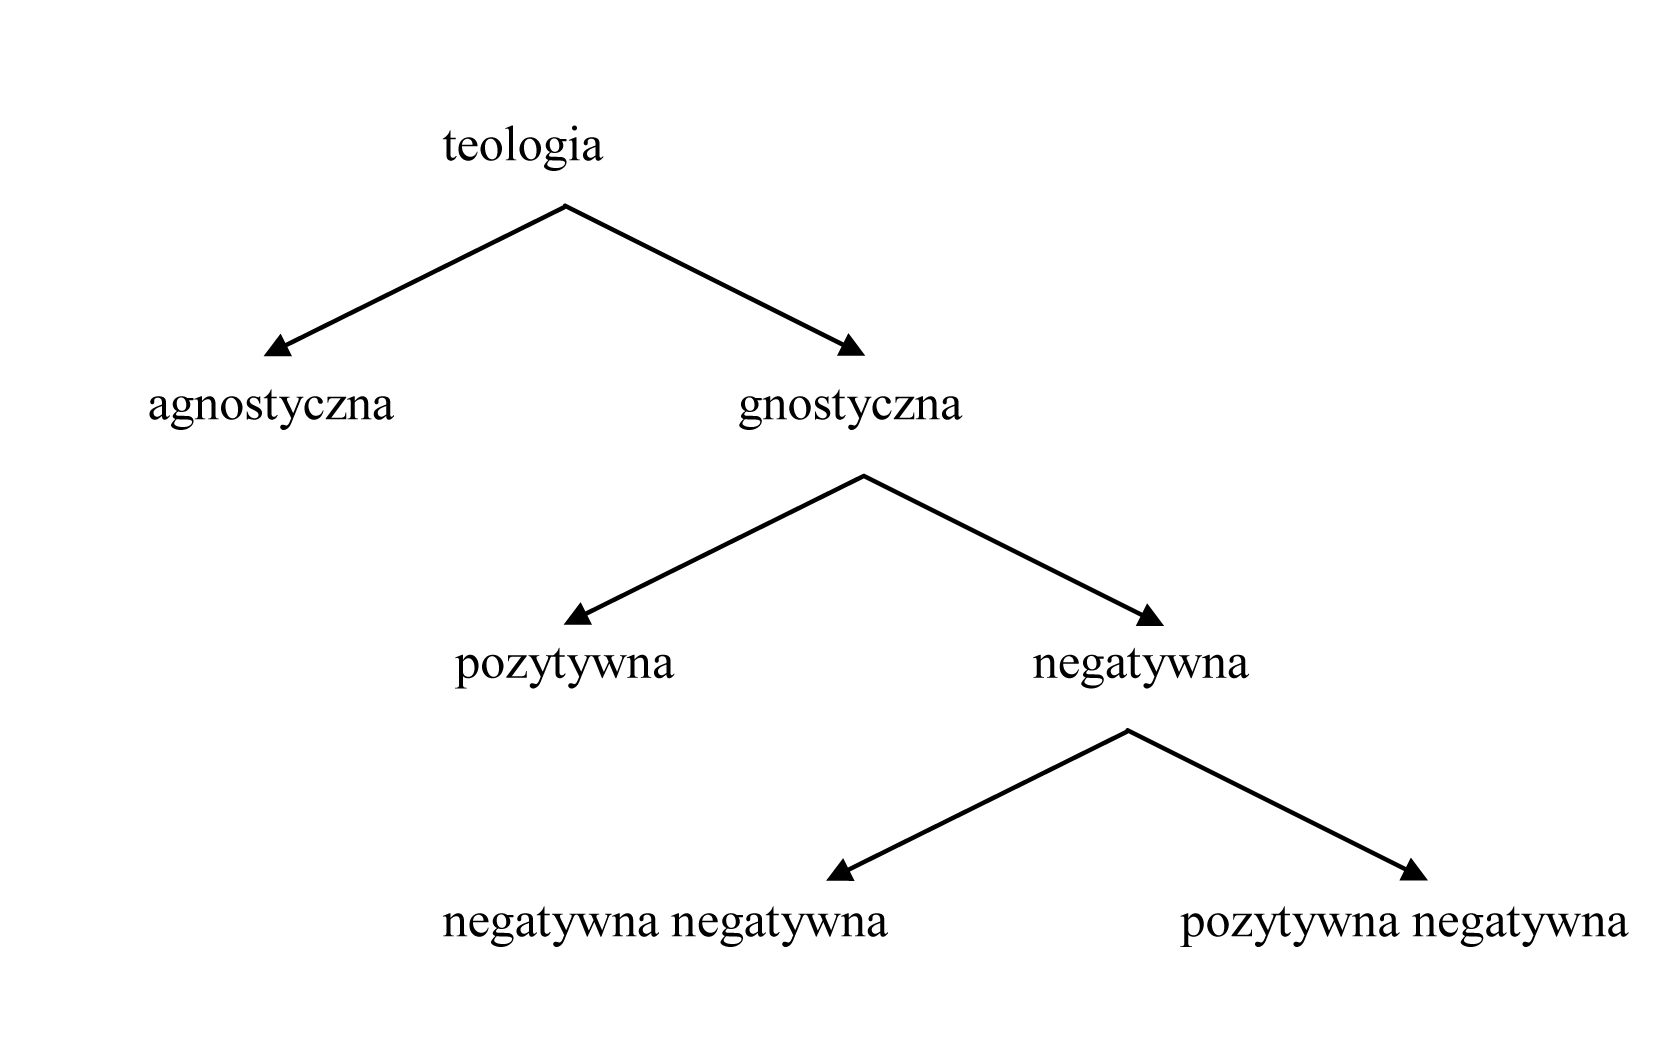
\includegraphics[width=1\linewidth]{typologia.jpg}
%\caption{Proponowana przez Rojka
%typologia interpretacji teologii apofatycznej.}
%}
%\end{figure}

%\begin{figure}[H]
%\begin{center}
% \begin{tikzpicture}[node distance=1cm]
%
%    \node (1) {teologia};
%    \node (21) [below=of 1, xshift=-2.5cm] {agnostyczna};
%    \node (22) [below=of 1, xshift=2.5cm] {gnostyczna};
%    \node (31b) [below=of 22, xshift=-2.5cm] {pozytywna};
%    \node (32b) [below=of 22, xshift=2.5cm] {negatywna};
%    \node (41) [below=of 32b, xshift=-2.5cm] {negatywna negatywna};
%    \node (42) [below=of 32b, xshift=2.5cm] {pozytywna negatywna};
%
%    \path[-] (1) edge (21);
%    \path[-] (1) edge (22);
%    \path[-] (22) edge (31b);
%    \path[-] (22) edge (32b);
%    \path[-] (32b) edge (41);
%    \path[-] (32b) edge (42);
%
%\end{tikzpicture}
%
%\caption[Typologia teologii apofatycznej według Rojka]{Proponowana przez Rojka
%typologia interpretacji teologii apofatycznej.}\label{roj-typ-rys}
%\end{center}
%\end{figure}

%Problemem, któremu Rojek poświęca nieco uwagi, lecz mimo wszystko
%postanawia go nie rozstrzygać, jest problem własności pozytywnych. Jest
%to problem poważny, ponieważ w świetle przedstawionej powyżej typologii
%różnica między teologią pozytywną i negatywną polega na orzekaniu o
%najwyższej istocie pozytywnych własności lub ich negacji. Jak
%zdefiniować zbiór takich własności? Rojek wymienia kryterium
%syntaktyczne, które miałoby polegać na ,,obecności negacji w
%predykacie''\footnote{Ibidem, s. 221. }. Nie do końca wiadomo, jak
%rozumieć takie kryterium. Przypuszczam, że formalnie można zapisać tę
%propozycję w logice predykatów II-rzędu w następujący sposób:
%
%\begin{equation}
%    P(Q) {=}_{df} \forall x \neg \exists N (Q(x) \equiv \neg N(x)),
%\end{equation}
%gdzie $P(Q)$ oznacza ,,własność $Q$ jest pozytywna''. Jednakże Rojek
%natychmiast dodaje, że kryterium syntaktyczne nie może być uważane za
%wystarczające. Powołuje się tu na klasyczny przykład predykatu ,,jest
%ślepy'' -- nie zawiera on negacji, lecz odnosi się do braku i z tego
%powodu wydaje się być pozytywny. Trafniejszym argumentem wydaje się być
%powołanie na św. Tomasza, wedle którego własności tradycyjnie
%przypisywane bytowi absolutnemu, takie jak prostota, doskonałość czy
%jedność, są w istocie własnościami negatywnymi\footnote{św. Tomasz z
%Akwinu Teologiczna: I, 3, Summa contra Gentiles 11. }.
%
%Problem własności pozytywnych Rojek pozostawia nierozwiązany tłumacząc,
%że skupia się na formie teologii negatywnej, nie na jej treści. Dodaje
%jednak, że istnieje jeszcze jeden bardzo szczególny sposób ich
%rozumienia. Można je traktować, jako najwyższy sposób istnienia danej
%własności, czyli tzw. perfekcje. Najczęściej mówi się o takich
%perfekcjach, jak wszechwiedza -- najwyższy sposób wiedzy, czy też
%wszechmoc -- najwyższy stopień mocy. Są one istotnym elementem w
%ontologicznych dowodach istnienia Boga, które w historii były
%proponowane m.in. przez św. Anzelma, Kartezjusza, Leibniza, Gödla i
%Perzanowskiego. W tych argumentach Boga można uznać za podmiot
%wszelkich własności pozytywnych rozumianych jako perfekcje:
%
%\begin{equation}
%    G(x) \equiv \forall Q (P(Q) \to Q(x)).
%\end{equation}
%
%
%Definicję tę Rojek zaczerpnął od Perzanowskiego\footnote{J.
%Perzanowski, Ontological Arguments II: Cartesian and Leibnizian, [w:]
%red. H. Burkhardt, B. Smith, Handbook of Metaphysics and Ontology, t.
%2, PhilosophiaVerlag, München 1991,ss.~625–633. } i stanowi ona
%wzór kolejnych definicji Boga w proponowanych przez niego następnie
%interpretacjach teologii negatywnej. Warto wiec poświęcić jej nieco
%uwagi. Po pierwsze, jest ona zapisana w rachunku predykatów drugiego
%rzędu, gdyż zawiera warunek, że własności przypisywane Bogu muszą być
%pozytywne. Po drugie, Bóg formalizowany jest jako predykat (,,$x$ jest
%Bogiem'', ,,$x$ jest bogopodobny''), nie jako stała logiczna\footnote{Por.
%choćby M. Durrant, The ,,Meaning of ‘God’-I, Royal Institute of
%Philosophy Supplement,vol. 31 (1992), ss. 71-84. }, lub deskrypcja
%określona, co proponował Bocheński\footnote{J.M. Bocheński\index[names]{Bocheński, Józef Maria}, op. cit.,
%s. 381. }. Po trzecie, powyższa definicja powstała na użytek
%formalizacji dowodów ontologicznych, które należą raczej do jakiejś
%formy teologii pozytywnej. Zawarte w niej $P(Q)$ czytamy jako ,,$Q$ jest
%własnością pozytywną'' w pewnym szczególnym sensie opisanym powyżej -- ,,$Q$
%jest perfekcją''. Rojek nie sugeruje jednak, że w teologii apofatycznej
%Pseudo-Dionizego zaprzecza się jedynie tego typu własnościom
%pozytywnym. Przeciwnie, pisze wprost, że zakres negowanych własności
%jest szerszy\footnote{P. Rojek, op. cit., s. 222. }. Po raz
%kolejny jednak odżegnuje się od określenia, o jakie konkretnie
%własności chodzi. Jest to, moim zdaniem, jeden z najsłabszych punktów
%jego propozycji. Wrócę do tego ponownie w dyskusji.


\section{Agnostyczna teologia negatywna}\label{roj-agnostycna}

Strategią pierwszej przedstawianej przez Rojka\index[names]{Rojek, Paweł} apofatycznej teorii Boga
jest przyjęcie \eqref{rojek-T4} jako tezy podstawowej i odrzucenie lub
modyfikacja pozostałych tez, za cenę zachowania spójności.
Jak już ujawniliśmy, celem tego typu doktryny jest podkreślenie znaczenia
boskiej transcendencji -- teoria ta głosi, że Bóg jest zasadniczo niewyrażalny
i~niepojmowalny. Takie rozumienie teologii negatywnej jest popularne wśród wielu
komentatorów -- także tych, którzy rozważają logiczno-językową strukturę
tej teorii\footnote{Wśród nich Rojek\index[names]{Rojek, Paweł} wymienia Jerome'a Gellmana\index[names]{Gellman, Jerome I.}, Johna J.
Jonesa\index[names]{Jones, John J.} oraz Paula Rorema\index[names]{Rorem, Paul}. Zob., odpowiednio, rozdz. \ref{sil-gell} oraz \ref{sil-dionizy}.}.

%W rozważaniach Gellmana teologia negatywna jest teorią, w której
%jakikolwiek predykat P języka ,,skończonych bytów'' nie może być
%przedziwie orzekany o Bogu. Jej główną tezą jest, że Bóg nie należy do
%zakresu żadnego z predykatów naszego języka. Jeśli mówimy na przykład,
%że Bóg nie jest mądry, mamy na myśli raczej negacją
%\textit{wykluczającą}, niż negację \textit{wyboru}. Naszym zamiarem
%jest wyłącznie stwierdzenie, że to nieprawda, że predykat P przysługuje
%Bogu, niekoniecznie sugerując, że można o nim orzec dopełnienie tego
%predykatu, czyli nie-P\footnote{J.I. Gellman, The Meta-Philosophy of
%Religious Language. ,,No\^us'', nr 11 (1971), s. 158. }. Według
%Gellmana, zdanie ,,Bóg jest potężny'' teolog negatywny zrozumie jako
%negację dopełnienia predykatu ,,jest potężny''. W innym kontekście
%oznaczałoby to przypisanie obiektowi, o którym mowa, tej właśnie
%własności. Jednakże w przypadku Boga negowanie dopełnienia predykatu P
%nie oznacza przypisywania mu P. Mówiąc ogólnie, zdania języka
%religijnego negują dopełnienia wszystkich wymienianych przez nie
%własności Boga, który jest poza zakresem wszystkich naszych predykatów.
%One, z kolei -- będąc predykatami języka skończonych bytów -- z
%konieczności muszą oznaczać niedoskonałe własności\footnote{Zob.
%Ibidem. }.
%
%Według Jonesa, teologia negatywna Pseudo-Dionizego Areopagity jest w
%dużej mierze teologią krytyczną. Polemizuje ona z błędnym sposobem
%mówienia o Bogu -- takim, który traktuje Go jak byty, czyli rzeczy lub
%pojęcia\footnote{J.J. Jones, op. cit., s. 357. }. Fakt, że Bóg
%przekracza wszelki byt, nadaje również strukturę językowi dyskursu
%teologicznego. Nie idzie tylko o to, że przypisywanie Bogu
%jakichkolwiek przymiotów przysługujących bytom jest z gruntu błędne.
%Zwykle, gdy mówimy o rzeczach, twierdzenia i przeczenia sprzeciwiają
%się sobie. W wykładni Dionizego nie dzieje się tak w przypadku Boga.
%Bóg nie jest jednym z bytów, zatem język służący do opisu bytów nie
%jest dla Niego właściwy. W wypracowanym przez niego języku teologicznym
%twierdzenia i zaprzeczenia należą do odmiennych grup, tworząc odmienne
%sposoby mówienia o Bogu. Ponieważ funkcjonują one w odmienny sposób,
%nie należy ich ze sobą mieszać. Te pierwsze przedstawiają Boga jako
%przyczynę wszystkiego, te drugie wyrażają jego transcendencję. Oba
%sposoby mówienia można stosować naraz zarówno do opisu Boga, jak i
%opisu przedmiotów, jednakże w ten sposób nie zdołamy wyrazić
%unikalności Boga -- tego, że jest czymś odrębnym od wszystkich
%bytów\footnote{Zob. Ibidem, s. 360. }. Możemy tego dokonać
%wyłącznie przez negację, która według Jonesa jest kluczowym punktem
%myśli Dionizego. Istotnym jest, że Jones wyraźnie odróżnia negację od
%zaprzeczenia.
%
%
%\begin{quote}
%        W przeciwieństwie do zaprzeczenia, negacja odnosi się do (nie)możliwości
%poznania i powiedzenia czegokolwiek o Bogu. Jest to, jeśli można tak
%powiedzieć, reguła drugiego rzędu posługiwania się nazwami pierwszego
%rzędu.\footnote{Ibidem, s. 381. Większą część tego cytatu podaję za
%Rojkiem, op. cit., s. 222. }
%\end{quote}






%Najbardziej agnostyczną interpretację Dionizyjskiej\index[names]{Pseudo-Dionizy Areopagita} teologii negatywnej
%zaproponował Paul Rorem. Podkreśla on podobieństwo teologii
%Pseudo-Dionizego z późną filozofią neoplatońską. W obu tych doktrynach
%byty uporządkowane są względem pewnej hierarchii i w celu dotarcia do
%bytu absolutnego należy ,,wspiąć się'' po tej ,,drabinie'' bytów. By
%spotkać Boga należy wpierw zanegować nasze wrażenia i wyobrażenia i
%przekroczyć je, by dojść do ich pojęciowych znaczeń. Następnie
%zanegowane zostać powinny także owe znaczenia oraz wszelkie inne
%pojęcia umysłu, ponieważ przekroczenie naszej wiedzy prowadzi do
%niepoznawalnego, do cichego zjednoczenia z Bogiem. Innymi słowy, Rorem
%zwraca uwagę, że u Areopagity drogą do Boga jest zaprzeczenie
%wszystkich bytów. Dionizy jednak wielokrotnie stwierdza, że Bóg jest
%także ponad wszelkim zaprzeczeniem. Ostatecznie więc, należy zanegować
%także wszelkie negacje, nie pozostawając już żadnym pojęciem
%Boga\footnote{Por. P. Rorem, Pseudo-Dionysius. A Commentary on the
%Texts and an Introduction to Their Influence, Oxford University Press,
%Oxford -- New York 1993, ss. 210-211. }. Jak zauważa Rorem, Dionizy
%,,zaprzecza i wykracza poza wszystkie nasze pojęcia lub «pojęciowe»
%atrybuty Boga i kończy na odrzuceniu wszelkiego mówienia i myślenia,
%nawet negatywnego''\footnote{Tenże, przypis do Pseudo-Dionizy
%Areopagita, The Complete Work, tłum. C. Luibheid,. Paulist Press, New
%York 1987, s. 99. Cytuję za P. Rojek, op. cit. }.





Wynikiem agnostycznej
interpretacji teologii negatywnej nie jest zatem twierdzenie, że Bóg posiada
własności negatywne. Stosunek Boga do własności -- czy to pozytywnych, czy negatywnych -- jest tu irrelewantny lub raczej niemożliwy do określenia. Główną tezą tej doktryny jest właśnie twierdzenie, że Bóg jest niewyrażalny i~niepoznawalny. 
Zgodnie ze wskazaną w~ten sposób dwuznacznością tezy \eqref{rojek-T4},
Rojek\index[names]{Rojek, Paweł} wyróżnia dwie wersje tej teorii. Wedle pierwszej z nich, Bóg jest
niewyrażalny, nie sposób go wysłowić.
%Konsekwentnym rozwinięciem tej
%teorii jest stwierdzenie, że dyskurs religijny jest pozbawiony
%jakiegokolwiek znaczenia.
Wedle drugiej wersji, Bóg jest
niepoznawalny, nie można posiąść o nim wiedzy.
%I choć dyskurs religijny
%posiada w tej teorii jakieś znaczenie, może on opisać wyłącznie to,
%czego o Bogu nie wiemy. Rojek omawia obie wersje tej interpretacji.
A zatem poruszamy się tutaj na gruncie dobrze nam znanej teologii milczenia, choć po raz pierwszy wyraźnie zaznaczony zostaje
wątek związany z niepoznawalnością Boga. Jak przekonuję w kolejnej części pracy\footnote{Zob. rozdz. \ref{scep-werapo}.}, teorię Niepoznawalnego należy
uważać za odrębną interpretacje teologii negatywnej. Umieszczenie tego fragmentu analiz Rojka\index[names]{Rojek, Paweł} w niniejszym rozdziale posiada jednak dodatkowe motywacje.
Po pierwsze, model tej teorii jest dla Rojka\index[names]{Rojek, Paweł} inspiracją w~budowaniu logicznej ramy dla jego własnej interpretacji -- pozytywnej teologii negatywnej. Bez przedstawienia sposobu, w~jaki Rojek\index[names]{Rojek, Paweł} dochodzi do logicznej rekonstrukcji teorii Niepoznawalnego, sprawozdanie z jego oryginalnego modelu straciłoby na jasności.
Po drugie, w~apofatycznej doktrynie Pseudo-Dionizego Areopagity\index[names]{Pseudo-Dionizy Areopagita}, która jest źródłem tez \eqref{rojek-T1}-\eqref{rojek-T4}, będących podstawą wszystkich rozważanych w niniejszym rozdziale teorii Boga, różnica między jego niewysławialnością a niepoznawalnością nie jest wyraźnie zarysowana.
Po trzecie, dosyć nietypowa syntaktyka zaproponowana przez Rojka\index[names]{Rojek, Paweł} do formalizacji teorii Niepoznawalnego nie posiada jednoznacznie epistemicznej natury, a~jej filozoficzne motywacje i~charakterystyka zdradzają symptomy świadczące, że w~tym przypadku wciąż pozostajemy na gruncie teologii milczenia.
W~końcu, do tego samego wniosku prowadzą nas Rojka\index[names]{Rojek, Paweł} komentarze do modelu teorii Niepoznawalnego, według których niepoznawalność Boga polega na niemożliwości \textit{twierdzenia}, że posiada on pozytywne własności.




\subsubsection{Teoria Niewysławialnego}\label{rojek-bochenski}

Teorię Niewysławialnego Rojek\index[names]{Rojek, Paweł} charakteryzuje zgodnie z duchem prezentowanej w~niniejszej części pracy teologii milczenia. Poprawnie identyfikuje jej paradoksalny charakter mający swe źródła w~samozwrotności.
Do jej rekonstrukcji adaptuje metajęzykowe ujęcie zaczerpnięte od Bocheńskiego\index[names]{Bocheński, Józef Maria}. Z~tego względu podstawową dla tej interpretacji teologii negatywnej tezę \eqref{rojek-T4} oddaje za Bocheńskim\index[names]{Bocheński, Józef Maria} jako
\begin{flalign*}
&G(x) \equiv \forall \mathcal{L}\ N_w(x,\mathcal{L}).&\tag{MNT''}\label{rojek-MNTbis}
\end{flalign*}

Rojek\index[names]{Rojek, Paweł} wydaje się być usatysfakcjonowany ustaleniami Bocheńskiego\index[names]{Bocheński, Józef Maria} i przekonany, że ujęcie teologii milczenia w postaci \ref{rojek-MNTbis} ratuje tę teorię przed sprzecznościami\footnote{Jak pokazałem w poprzednim rozdziale (rozdz. \ref{sil-boch-dyskusja}), można mieć co do tego wątpliwości.}.
Powyższą formułę wraz dodatkowymi uwagami głoszącymi, że mamy tu do czynienia z~wypowiedzią metajęzykową, nazywa ,,modelem'' teorii Niewysławialnego. Przyjmuje też w pełni Bocheńskiego\index[names]{Bocheński, Józef Maria} argumenty przeciwko teorii Niewysławialnego -- fakt, że nie możemy przypisać Bogu żadnej własności przedmiotowo-językowej sprawia, że teoria ta jest niezgodna z faktycznym dyskursem religijnym i religijną \textit{praxis}, a~więc dyskwalifikuje ją jako poprawną teorię Boga. Ze względu na jej uwikłanie w~swoje ,,zewnętrzne'' paradoksy należy ją odrzucić.



%Podobnie argumentuje John Hick, który uważa, że nie ma sensu
%
%
%\begin{quote}
%mówić o X, że żadne nasze pojęcie się do niego nie stosuje. Jest bowiem
%w oczywisty sposób niemożliwe odnosić się do czegoś, co nie posiada
%nawet własności 'bycia możliwym przedmiotem
%odniesienia.\footnote{J. Hick, An Interpretation of Religion. Human
%Responses to the Transcendent, Yale University Press, New Haven –
%Londyn 1989, s. 239. Cytuję za P. Sikora, Logos Niepojęty, Wydawnictwo
%Universitas, Kraków 2010, s. 118. }
%\end{quote}
%
%
%Dodaje on także, że określenie
%
%\begin{quote}
%,,taki, że nasze pojęcia się do niego nie stosują'' nie może,
%jeśli chcemy uniknąć paradoksu, odnosić się do własności, którą
%opisuje.\footnote{Ibidem. }
%\end{quote}
%
%Przeciwko takiemu przedstawianiu teorii Niewysławialnego występuje Józef
%Maria Bocheński. Twierdzi on, że da się ją uratować od sprzeczności,
%lecz nawet mimo tego, nie odpowiada ona potrzebom dyskursu
%religijnego\footnote{Zob. J.M. Bocheński, op. cit., ss. 353-356.
%}. Bocheński uważa, że jeśli przestrzega się pewnych obowiązujących w
%logice konwencji, zarzut sprzeczności stawiany teorii Niewysławialnego
%przestanie obowiązywać. Należałoby wpierw dowieść, że danym układzie
%odniesienia teoria ta prowadzi do sprzeczności, tymczasem nikt takiego
%dowodu nie przedstawił. Według Bocheńskiego sytuacja przedstawia się
%zupełnie przeciwnie -- nietrudno wykazać, że teoria Niewysławialnego
%jest spójna. Poniżej przedstawię jego argumentację.
%
%Załóżmy, że dwuargumentowy predykat  $Nw(x,l)$ oznacza ,,$x$ jest
%niewyrażalne w języku $l$''.
%
%Zapiszmy teraz formułę zawierającą ten predykat
%
%\begin{equation}
%    \exists x \exists l Nw(x, l)
%\end{equation}
%
%
%Wydaje się, że nie tylko można ją wypowiedzieć nie popadając w
%sprzeczność, lecz także jest ona prawdziwa, nietrudno znaleźć taki
%obiekt $x$ i taki język $l$, które spełniałyby zapisany wyżej warunek.
%(Bocheński podaje przykład krowy i języka szachów: nie da się opisać
%krowy w języku szachów).
%
%Możemy powyższy przykład uogólnić i sformułować metajęzykową definicję
%Boga o następującej postaci:
%
%\begin{equation}\tag{G2}
%    G(x) \equiv \forall l Nw(x, l)\footnote{Definicję podaję za
%Rojkiem, różni się ona od zapisu Bocheńskiego tym, że u tego ostatniego
%,,Bóg'' zapisany został jako stała logiczna: $\forall l Nw(a, l)$.}
%\end{equation}
%
%
%
%Na pierwszy rzut oka, wydaje się, ze ta formuła jest bardziej
%problematyczna -- twierdzenie, że $x$ jest niewysłowione w żadnym języku
%zdaje się prowadzić do sprzeczności. Można jednak uniknąć tego
%problemu, stosując zwykłe konwencje wykorzystywane do pozbywania się
%antynomii semantycznych. Należy założyć, że żadne zdanie traktujące o
%pewnej klasie języków, nie jest formułowane w żadnym z tych języków.
%Aby było pozbawione sprzeczności musi zostać sformułowane w innym
%języku, czyli odpowiednim metajęzyku. Możemy więc założyć, że klasa
%języków wspominana w (G2) jest klasą języków przedmiotowych. W takim
%wypadku (G2) jest zdaniem metajęzyka pierwszego stopnia. Po takim
%zabiegu, sformułowana definicja jest znacząca i pozbawiona
%sprzeczności. Nie ma bowiem niespójności w twierdzeniu, że coś nie daje
%się wysłowić w jakimś języku, lub nawet w klasie języków, o ile
%twierdzenie to jest w języku nienależącym do tej klasy. Według
%Bocheńskiego, przy takim założeniu, standardowym z punktu widzenia
%logiki ogólnej, teoria Niewysławialnego pozostaje znacząca i spójna a
%zarzut sprzeczności zostaje oddalony.
%
%Bocheński odrzuca jednak teorię Niewysławialnego z co najmniej dwóch
%powodów. Po pierwsze, na mocy (G2) nie można przypisać Bogu
%jakiekolwiek własności językowo przedmiotowej. Jedyną własnością, jaką
%możemy mu przypisać, jest metajęzykowa własność bycia niewysłowionym w
%żadnym z języków przedmiotowych. W takim wypadku wierny, nie mógłby
%akceptować żadnego zdania dyskursu religijnego, które przypisałoby Bogu
%jakąkolwiek własność-przedmiotowo-językową. Wydaje się to niespójne z
%faktycznym dyskursem religijnym. Po drugie, niemożliwe byłoby oddawanie
%czci obiektowi, o którym wiemy tylko i wyłącznie, że nie można o nim
%nic powiedzieć. Jeśli wierny miałby czcić obiekt pozbawiony własności
%przedmiotowo-językowych, równie dobrze tym obiektem mógłby nie być Bóg
%a szatan\footnote{Por. J.M. Bocheński, op. cit., ss. 354-356. }.

%Rojek dodaje do tego podobny argument, jednakże umieszczony w kontekście
%teologii negatywnej. Mianowicie, jeśli teoria Niewysławialnego ma być
%właściwą interpretacją teologii negatywnej, można poddać w wątpliwość
%zasadność jednoczesnego utrzymywania tez \eqref{rojek-T1}-\eqref{rojek-T3}. Jeśli Bóg jest
%niewyrażalny, cały język religijny jest pozbawiony znaczenia, nie
%możemy więc ani sensownie potwierdzić, ani zaprzeczyć żadnym z Jego
%własności. Dla Rojka jest to wskazówka, by \eqref{rojek-T4} nie interpretować
%semantycznie, lecz epistemologicznie lub nawet
%ontologicznie\footnote{Zob. P. Rojek, op. cit., s. 223.}. W ten sposób przechodzi od
%teorii Niewysławialnego do agnostycznej teorii Niepoznawalnego.

Rojek\index[names]{Rojek, Paweł} dodaje do tego argument sformułowany w kontekście
swoich analiz. Mianowicie, jeśli teoria Niewysławialnego ma być
właściwą interpretacją teologii negatywnej, należy podać w wątpliwość
zasadność utrzymywania tez \eqref{rojek-T1}-\eqref{rojek-T3}. Jeśli Bóg jest
niewyrażalny, cały język religijny jest pozbawiony znaczenia, nie
możemy więc ani sensownie potwierdzić, ani zaprzeczyć żadnym z jego
własności. Krótko mówiąc, teoria Niewysławialnego zdaje się nie dawać żadnych szans na
akceptację którejkolwiek z wyabstrahowanych tez teologii apofatycznej poza \eqref{rojek-T4}.
Dla Rojka\index[names]{Rojek, Paweł} jest to wskazówka, by nie interpretować tej tezy
semantycznie, lecz epistemologicznie lub nawet
ontologicznie\footnote{Zob. P. Rojek, \textit{Logika teologii negatywnej}, op. cit., s. 223.}. W ten sposób przechodzi od
teorii Niewysławialnego do agnostycznej teorii Niepoznawalnego.


\subsubsection{Agnostyczna teoria Niepoznawalnego}

Według Rojka\index[names]{Rojek, Paweł} teoria Niepoznawalnego jest lepszym modelem teologii apofatycznej,
ponieważ nie tylko przyjmuje \eqref{rojek-T4} za twierdzenie podstawowe, lecz także
umożliwia pewną interpretację tez \eqref{rojek-T2} oraz \eqref{rojek-T3}. By to pokazać,
wprowadza pojęcie nieokreśloności oraz definiuje nowe, odmienne od
klasycznego pojęcie negacji. W tym celu wykorzystuje on logiczną teorię
nieokreśloności, którą na potrzeby modelowania (w~filozofii) nauki rozwinął
rosyjski logik Aleksander Zinowjew\index[names]{Zinowjew, Aleksander}\index[names]{Zinowjew, Aleksander}\footnote{A.A. Zinov'ev, \textit{Foundations
of the Logical Theory...}, op. cit. Zob. także idem,
\textit{Logika nauki}, op. cit. }.

Filozoficzną motywacją logiki Zinowjewa\index[names]{Zinowjew, Aleksander} są  pewne ,,nieklasyczne'' przypadki
spotykane w teoriach i wynikach naukowych oraz ich interpretacjach, w których zniesione zostaje
prawo wyłączonego środka. Takie przypadki polegają na dopuszczeniu
możliwości istnienia obiektów, co do których nie da się ustalić, czy
posiadają one jakąś własność $Q$, czy też posiadają własność
$\neg Q$. Można do nich zaliczyć na przykład rozważaną
w~mechanice kwantowej cząstkę elementarną, której parametry -- zgodnie z
zasadą nieoznaczoności~-- nie mogą zostać ustalone\footnote{Interesujące może okazać się zbadanie związków pewnych rozwiązań wypracowanych w~ramach
teologii negatywnej
oraz filozofii mechaniki kwantowej.
Tym, którzy podają w wątpliwość teoretyczną wartość teologii negatywnej,
istnienie innych obszarów, w których możliwości ludzkiego języka i pojęć zdają się być niewystarczające, może dostarczyć argumentu
na rzecz wiarygodności tej doktryny jako teologicznej teorii tego, nie niewysławialne i niepojmowalne.
},
twierdzenie, które
na gruncie danego rachunku logicznego nie może zostać ani dowiedzione,
ani obalone, albo po prostu obiekt zmieniający się w~czasie. Na
potrzeby takich przypadków Zinowjew\index[names]{Zinowjew, Aleksander} nad logiką klasyczną wprowadza nowy funktor nieokreśloności i
oznacza go symbolem $?$\footnote{Dla utrzymania spójności zapisu, formuły teorii
nieokreśloności Zinowjewa\index[names]{Zinowjew, Aleksander} przedstawiam w~nieco zmodyfikowanej notacji zaproponowanej przez
Rojka\index[names]{Rojek, Paweł}.}. Niech zapis $?Q(x)$ oznacza ,,nie można
ustalić, czy $x$ ma $Q$, czy $x$ ma nie-$Q(x)$'', co można czytać także jako ,,$x$ ma w sposób
nieokreślony $Q$''. W~teorii Niepoznawalnego Bóg uznawany jest za
obiekt, którego nie da się poznać. Rojek\index[names]{Rojek, Paweł} proponuje, by za pomocą powyższego funktora nieokreśloności z logiki Zinowjewa\index[names]{Zinowjew, Aleksander}
podać nową definicję Boga jako obiektu, który wszystkie pozytywne
własności posiada w~sposób nieokreślony.
\begin{flalign*}
&G(x) \equiv \forall Q (P(Q) \to ?Q(x)).&\tag{ZNT}\label{rojek-ZNT}
\end{flalign*}
%\begin{equation}\tag{G3}
%   G(x) \equiv \forall Q (P(Q) \to ?Q(x)).
%\end{equation}

%
%
%Formule tej należy poświęcić nieco uwagi. Po pierwsze, w odróżnieniu od
%\ref{sil-boch-MNT} powyższa definicja nie jest wyrażona w metajęzyku, lecz w języku
%przedmiotowym. Po drugie, co istotniejsze, by uniknąć kłopotów z
%formalizowaniem Boga przy użyciu predykatu $G(x)$, należy ją ograniczyć.
%Do tej definicji trzeba dołożyć dodatkowe założenie, o postaci:
%
%\begin{equation}
%    \neg P(G)
%\end{equation}
%
%
%Innymi słowy, należy założyć, że predykat ,,jest Bogiem'' (lub ,,jest
%bogopodobny'') nie należy do zbioru predykatów pozytywnych. W
%przedziwnym bowiem razie, wpadlibyśmy w błędne koło i o niczym nie
%można byłoby określić, że jest Bogiem.

Jak twierdzi Rojek\index[names]{Rojek, Paweł}, wykorzystując ten formalizm do modelowania teorii
Niepoznawalnego, można -- w pewnym szczególnym sensie -- zaprzeczyć, że
Bóg posiada wszystkie własności pozytywne.
%Oczywiście, nie idzie tutaj
%o stwierdzenie, że o Bogu można na orzec jakiekolwiek
%$\neg Q$, przy założeniu, że $Q$ jest własnością pozytywną.
%Taki przypadek jest niezgodny zasadą \ref{rojek-ZNT}.
Idzie o to, że po
wprowadzeniu funktora nieokreśloności $?$, zdanie
,,nieprawda, że $x$ jest
$Q$''\footnote{Rojek mówi o wyrażeniu ,,$x$ jest nie-$Q$'', moim zdaniem
błędnie. W ogóle w przedstawieniu teorii Niepoznawalnego w szacie logiki nieokreśloności Zinowjewa\index[names]{Zinowjew, Aleksander} odnaleźć można dużo niezgrabności. Por. P.~Rojek, \textit{Logika teologii negatywnej}, op. cit., s.~223. Kładę to jednak na karb nietypowej notacji stosowanej przez radzieckiego logika, którą Rojek\index[names]{Rojek, Paweł} próbuje przeredagować według bardziej współczesnych standardów.} staje się dwuznaczne. Może ono przyjąć jedno
z dwóch znaczeń: albo ,,$x$ jest nie-$Q$'', albo ,,nie można stwierdzić, czy $x$~jest~$Q$''. W nomenklaturze Rojka\index[names]{Rojek, Paweł}, w pierwszym przypadku w~zdaniu pojawia
się negacja w~znaczeniu \textit{de dicto}, o~drugim znaczeniu natomiast
można mówić, że zawiera ono negację \textit{de re}. Nieco inne
nazewnictwo wprowadził Zinowjew\index[names]{Zinowjew, Aleksander}, który pierwszy rodzaj negacji nazwał
negacją zewnętrzną -- odnosi się ona bowiem do całego negowanego w~ten
sposób zdania, drugą negację nazwał
negacją wewnętrzną -- dotyczy ona bowiem wyłącznie predykatu\footnote{Konkretnie: operatora predykatywności.
Notacja zaproponowana przez Rojka\index[names]{Rojek, Paweł} pozbawiona jest już symbolu takiego operatora.}.

Przyjmijmy teraz dwa różne symbole, w celu odróżnienia odmiennych pojęć
negacji. Niech $\neg$ oznacza negację zewnętrzną,
natomiast symbol $\sim$ negację wewnętrzną. Przy
takiej notacji, formułę ${\sim}Q(x)$ czytamy jako ,,$x$ jest
nie-$Q$'', lub  inaczej: ,,$x$ ma własność nie-$Q$''\footnote{U Rojka\index[names]{Rojek, Paweł}: ,,$x$ ma
własność $\neg Q$''. }, natomiast formuła
$\neg Q(x)$\footnote{Rojek używa tych symboli na odwrót, to jest $\neg$ stosuje na oznaczenie negacji
wewnętrznej, a~$\sim$~używa do oddania negacji zewnętrznej. Dodatkowo formułę negowaną za pomocą
funktora negacji zewnętrznej opatruje w dodatkowe nawiasy po to, by
podkreślić odmienny, ,,zewnętrzny'' charakter tego rodzaju negacji.
Uznaję ten zabieg za redundantny i niekonieczny. Notacja Rojka\index[names]{Rojek, Paweł} jest odmienna od
stosowanej oryginalnie przez Zinowjewa\index[names]{Zinowjew, Aleksander}.} oznacza ,,nieprawda, że $x$~jest $Q$'', lub ,,nie twierdzi się, że
$x$~ma własność $Q$''. Poniższe aksjomaty definiują relacje, jakie zachodzą
pomiędzy funktorem nieokreśloności a funktorami negacji wewnętrznej i~zewnętrznej\footnote{Aksjomaty podaję za Rojkiem\index[names]{Rojek, Paweł}, bez żadnej kwantyfikacji i konsekwentnie trzymam się tej konwencji.}:
\begin{flalign*}
&\neg Q(x) \equiv {\sim} Q(x)\ \lor\ ?Q(x),&\tag{Z\textsubscript{1}}\label{rojek-zin1}\\
&\neg {\sim} Q(x) \equiv Q(x)\ \lor\ ?Q(x),&\tag{Z\textsubscript{2}}\label{rojek-zin2}\\
&\neg ?Q(x) \equiv Q(x)\ \lor\ {\sim} Q(x)  .&\tag{Z\textsubscript{3}}\label{rojek-zin3}
\end{flalign*}
%\begin{equation}\tag{Z1}
%\neg  Q(x) \equiv ?Q(x) \lor {\sim} Q(x),
%\end{equation}
%\begin{equation}\tag{Z2}
%\neg {\sim} Q(x) \equiv Q(x)\ \lor\ ?Q(x),
%\end{equation}
%\begin{equation}\tag{Z3}
%\sim ?Q(x) \equiv Q(x) \lor {\sim} Q(x).
%\end{equation}
Z \eqref{rojek-zin3} oraz prawa De Morgana\index[names]{De Morgan, Augustus} bezpośrednio wynika:
\begin{flalign}
& ?Q(x)\ \equiv\ \neg  Q(x)\ \land\ \neg {\sim} Q(x). &\label{rojek-zin4}
\end{flalign}
%\begin{equation}
%   \vdash \quad ?Q(x)\ \equiv\ \neg  Q(x)\ \land\ \neg {\sim} Q(x).
%\end{equation}
 



Gdybyśmy chcieli dokonać kolapsu z powrotem do logiki klasycznej,
musielibyśmy założyć, że (dla każdego $x$, dla dowolnego $Q$) zachodzi $\neg ? Q(x)$. Prawdziwe jest bowiem twierdzenie

\begin{flalign}
&  \neg ?Q(x)\ \to \big({\sim} Q(x) \equiv \neg Q(x)\big).&
\end{flalign}
Przy założeniu, że nie istnieją przypadki nieokreśloności, negacje \textit{de re} i \textit{de
dicto} stają się tożsame.
Jednakże, jeśli
chcemy opisać wspomniane wyżej przypadki nieklasyczne, w~których
posiadanie lub nieposiadanie danej własności przez jakiś obiekt
nie może zostać określone, musimy zgodzić się na obecność dwóch
różnych, nierównoważnych pojęć negacji w systemie. Z tego powodu
poniższa formuła nie jest wyprowadzalna w ramach prezentowanego tu systemu:
\begin{flalign}
& \nvdash  \neg  Q(x) \to  {\sim} Q(x). &
\end{flalign}
%
%\begin{equation}
%    \nvdash \quad \neg  Q(x) \to  {\sim} Q(x).
%\end{equation}
Dzieje się tak, ponieważ $\neg Q(x)$ pociąga za sobą ${\sim} Q(x)$ lub
$?Q(x)$. Analogicznie, w~prezentowanym tu rachunku nie zachodzi
następująca wersja prawa podwójnej negacji
\begin{flalign}
& \nvdash   \neg  {\sim} Q(x) \to  Q(x), &
\end{flalign}
%
%
%\begin{equation}
%   \nvdash   \neg  ({\sim} Q(\textit{x})) \to  Q(\textit{x}),
%\end{equation}
ponieważ $\neg {\sim} Q(x)$ implikuje $Q(x)$ lub $?Q(x)$. Prawdziwe są
natomiast następujące formuły:
\begin{flalign}
&   {\sim} Q(x) \to  \neg  Q(x), &\\
&   Q(x) \to  \neg  {\sim} Q(x). &
\end{flalign}


%\begin{equation}
%    \vdash \quad {\sim} Q(x) \to  \neg  Q(x),
%\end{equation}
%\begin{equation}
%    \vdash \quad Q(x) \to  \neg  {\sim} Q(x).
%\end{equation}






Należy zauważyć, że dla negacji wewnętrznej nie można mówić
o ,,nieklasycznym'' prawie wyłączonego środka
\begin{flalign}
& \nvdash  Q(x) \lor {\sim} Q(x), &
\end{flalign}
%
%\begin{equation}
%     \nvdash \quad Q(x) \lor {\sim} Q(x),
%\end{equation}
ponieważ istnieje dodatkowa, trzecia możliwość -- $?Q(x)$. Do grona tez tego
rachunku należy zatem następująca formuła:
\begin{flalign}
&    Q(x) \lor  {\sim} Q(x)\ \lor\  ?Q(x). &
\end{flalign}
%\begin{equation}
%    \vdash \quad Q(x) \lor  {\sim} Q(x) \lor  ?Q(x)
%\end{equation}
Prawo wyłączonego środka obowiązuje natomiast dla negacji \textit{de
dicto}:
\begin{flalign}
&    Q(x) \lor  \neg  Q(x), &\\
&    {\sim} Q(x) \lor  \neg  {\sim} Q(x), &\\
&    ?Q(x) \lor  \neg  ?Q(x). &
\end{flalign}
%\begin{equation}
%    \vdash \quad Q(x) \lor  \neg  Q(x),
%\end{equation}
%\begin{equation}
%    \vdash \quad {\sim} Q(x) \lor  \neg  {\sim} Q(x),
%\end{equation}
%\begin{equation}
%\vdash \quad ?Q(x) \lor  \neg  ?Q(x).
%\end{equation}

Niewątpliwym wkładem Rojka\index[names]{Rojek, Paweł} jest spostrzeżenie, że rachunek Zinowjewa\index[names]{Zinowjew, Aleksander} stworzony pierwotnie na potrzeby
logicznej rekonstrukcji  pewnych teorii naukowych, w~ramach których naruszona zostaje reguła \textit{tertium non datur}, może okazać się przydatny także do modelowania
omawianej w tym paragrafie interpretacji teologii apofatycznej. Dzięki
 własnościom tego rachunku, można przedstawić w sposób niesprzeczny już trzy spośród
tez wypreparowanych z pism Pseudo-Dionizego Areopagity\index[names]{Pseudo-Dionizy Areopagita}. Rekonstrukcją
tezy \eqref{rojek-T4} w~obrębie tej interpretacji i w terminach rachunku Zinowjewa\index[names]{Zinowjew, Aleksander} jest definicja Boga podana przez \ref{rojek-ZNT}.
Z tejże formuły, na podstawie praw logiki Zinowjewa\index[names]{Zinowjew, Aleksander} nietrudno już wyprowadzić dwie kolejne tezy doktryny Dionizego\index[names]{Pseudo-Dionizy Areopagita}.

Negację, o której mowa
w \eqref{rojek-T2}, można traktować jako negację \textit{de dicto}, ponieważ
zgodnie z teorią Niepoznawalnego, nie możemy stwierdzić, czy
Bóg posiada jakieś własności\footnote{Ten fragment analiz Rojka\index[names]{Rojek, Paweł} jest trochę naciągany. Związane jest to z~narzuceniem specyficznej interpretacji na funktor ,,zwykłej'', zewnętrznej negacji \textit{de dicto} jako ,,nie można stwierdzić, że'', podczas gdy taka interpretacja prędzej przysługiwałaby funktorowi nieokreśloności. Jednakże biorę to rozumienie za dobrą monetę, a~słabe punkty analiz Rojka\index[names]{Rojek, Paweł} wskażę w innych miejscach.}. W takim podejściu, \eqref{rojek-T2} stwierdza, że o
Bogu można orzec zewnętrzne negacje wszystkich własności pozytywnych. A
zatem, w języku tego rachunku należałoby to zapisać w następujący sposób:
\begin{flalign}
&    G(x) \to  (\forall Q (P(Q) \to  \neg Q(x)). &\tag{T2'}\label{rojek-T2prim}
\end{flalign}
%
%
%\begin{equation}
%    G(x) \to  (\forall Q (P(Q) \to  \neg Q(x)).
%\end{equation}
%
%
%
Co więcej, powyższa formuła jest bezpośrednią konsekwencją definicji
\ref{rojek-ZNT} i (\ref{rojek-zin4}). Ponieważ negacja
\textit{de dicto} jest różna od negacji \textit{de re}, nie możemy
jednocześnie twierdzić, że Bóg posiada (wewnętrzną) negację wszystkich
pozytywnych własności, czyli że można o~nim orzekać każde nie-$Q$, o ile
$Q$ jest pozytywne. Z~obu tych formuł wynika
także
\begin{flalign}
&    G(x) \to  (\forall Q (P(Q) \to
\neg {\sim} Q(x)), &\tag{T3'}\label{rojek-T3prim}
\end{flalign}
%
%\begin{equation}
%    G(x) \to  (\forall Q (P(Q) \to
%\neg {\sim} Q(x)),
%\end{equation}
%
%
którą Rojek\index[names]{Rojek, Paweł} uważa  za zrekonstruowaną w ramach syntaksy Zinowjewa\index[names]{Zinowjew, Aleksander} tezę \eqref{rojek-T3}.
Formuła ta zawiera
podwójne przeczenie, jednakże pierwsza negacja ma charakter \textit{de
dicto}, natomiast druga jest negacją \textit{de re}. Brzmieniem tej
formuły jest ,,Nieprawda, że Bóg posiada wszystkie wewnętrzne negacje
pozytywnych własności''.

W takim wypadku, wszystkie stwierdzenia Dionizego\index[names]{Pseudo-Dionizy Areopagita} o tym, że Bóg nie jest
ani $Q$, ani nie-$Q$, na przykład że nie jest on ,,ani wielkością, ani
małością, ani równością, ani nierównością, ani podobieństwem, ani
niepodobieństwem'', ,,nie jest też niczym z niebytu ani czymś z
bytu''\footnote{Pseudo-Dionizy Areopagita, \textit{Teologia mistyczna}, dz.
cyt., rozdział V. } itp.,  można niesprzecznie interpretować w
ramach powyższej rekonstrukcji. Podobnie wypowiedzi Areopagity\index[names]{Pseudo-Dionizy Areopagita} o
tym, że Bóg jest ,,ponad wszelkim twierdzeniem i~ponad wszelkim
zaprzeczeniem''\footnote{Ibidem.} można ująć w ramach
prezentowanego rachunku, jako koniunkcję warunków zawartych już
w~formułach \eqref{rojek-T2prim} i \eqref{rojek-T3prim}.
\begin{flalign}
&    G(x) \to  (\forall Q (P(Q) \to  \neg  Q(x) \land
\neg {\sim} Q(x)). &
\end{flalign}

%\begin{equation}
%    G(x) \to  (\forall Q (P(Q) \to  \neg  Q(x) \land
%\neg {\sim} Q(x)).
%\end{equation}



%Jak zauważa Rojek, istnieje wyjątek od konsekwentnego stosowania tej
%interpretacji. Nie można w ten sposób formalizować  twierdzeń, że Bóg
%nie jest ani poznawalny ani niepoznawalny, ani określony, ani
%nieokreślony. Taka treść predykatu $Q$ naraziłaby bowiem tę interpretację
%na sprzeczność. Jednakże wydaje się, że żadne z dzieł Dionizego nie
%zawiera podobnych sformułowań\footnote{Także Jones zauważa, że teza o
%niepoznawalności Boga ma wyjątkowy charakter w pismach Dionizego i
%nigdy nie występuje w podobnych parach. Zob. J.J. Jones, op. cit., s.
%358. }.


Rojek\index[names]{Rojek, Paweł} jest przekonany, że powyższe analizy chronią agnostyczną teologię negatywną przed
sprzecznościami, a~największą ich wadą jest to, że nie obejmują wszystkich tez wypreparowanych z pism Areopagity\index[names]{Pseudo-Dionizy Areopagita}.
Na tym gruncie teoria Niepoznawalnego wydaje się lepszą
interpretacją teologii negatywnej -- można w jej ramach
przyjąć aż trzy z apofatycznych tez. Teoria
Niewysławialnego ustępuje w tym zestawieniu  i obejmuje tylko jedną
tezę Dionizyjskiej\index[names]{Pseudo-Dionizy Areopagita} doktryny. Obie jednak zawodzą w interpretacji \eqref{rojek-T1}.
Teza ta nie znajduje swojego miejsca w agnostycznych 
interpretacjach, bowiem -- skoro Bóg jest niepoznawalny -- nie można o nim
nic sensownie stwierdzić.
Do tej uwagi Rojek\index[names]{Rojek, Paweł} dokłada argumenty Bocheńskiego\index[names]{Bocheński, Józef Maria} przeciw teorii Niewysławialnego -- tym razem stosując je do obu interpretacji w ramach agnostycznej teologii negatywnej.
Są one zasadniczo niespójne z faktycznym dyskursem
i praktyką religijną. Zgodnie z ich duchem, wierny nie mógłby
akceptować żadnych zdań dyskursu religijnego, które przypisują Bogu
jakieś własności. Tymczasem każdy dyskurs religijny zawiera
przynajmniej kilka takich zdań. Poza tym, gdyby o Bogu nie można było
orzekać żadnych własności, nie mógłby on być przedmiotem wiary i~czci\footnote{
Zob. J.M. Bocheński\index[names]{Bocheński, Józef Maria}, \textit{Logika religii}, op. cit., ss. 355-356, a~także rozdz. \ref{sil-boch-nonsens}.}.




\section{Negatywna teologia negatywna}

Wad tych pozbawiona jest druga interpretacja teologii negatywnej, którą
Rojek\index[names]{Rojek, Paweł} nazywa negatywną teologią negatywną. Jej punktem wyjścia jest
teza \eqref{rojek-T2}. Na gruncie tej interpretacji nie twierdzi się, że
dyskurs religijny pozbawiony jest znaczenia, ani że Bóg jest
niepoznawalny. Uważa się natomiast, że o przedmiocie religijnym można
orzekać wyłącznie negatywne własności. Nie jest więc tak, że nic nie
wiemy o Bogu -- wiemy, że nie posiada on pozytywnych własności.
%Należy
%przyznać, że jest to dość popularna interpretacja teologii
%apofatycznej. Na przykład, do właśnie w taki sposób rozumianej teologii
%negatywnej odnosił się Józef Maria Bocheński\index[names]{Bocheński, Józef Maria} w dziele \textit{Logika
%religii}.

%W analizie Rojka, negację obecną w \eqref{rojek-T2}
%należy traktować w~zwykły, klasyczny sposób. Zatem \eqref{rojek-T1} oraz \eqref{rojek-T3} muszą zostać natychmiast odrzucone, jako niespójne z tezą przyjętą tu za podstawową.
Z drugiej strony, wedle tej wersji teologii negatywnej, wszystko, co możemy orzec o~Bogu,
posiada ściśle negatywny charakter. Na tym ma polegać boska transcendencja.
Choć taka teoria zatraca swój samozwrotny charakter (obecny w jakimś
stopniu w agnostycznej teologii negatywnej), w jej analizach nietrudno wskazać innego rodziaju sprzeczności. W~obrębie tej interpretacji Bóg
wciąż pozostaje w jakimś
sensie niepoznawalny -- jedyne, co o Nim wiemy to jaki nie jest. Można
więc pokusić się także na próbę uwzględnienia tezy \eqref{rojek-T4} w ramach modelu tej teorii.

Rojek\index[names]{Rojek, Paweł} twierdzi, że w tym modelu teologii negatywnej właściwą definicją
Boga jest formalizacja tezy \eqref{rojek-T2} w obrębie klasycznego rachunku
predykatów drugiego rzędu.
Skoro mamy do czynienia z~klasyczną negacją, \eqref{rojek-T1} oraz \eqref{rojek-T3} muszą zostać natychmiast odrzucone jako niespójne z tezą przyjętą tu za podstawową.
Bóg -- analogicznie do poprzednich definicji –
opisany jest jako obiekt, o którym można orzekać negacje wszystkich
pozytywnych własności:
\begin{flalign}
&    G(x) \equiv  \forall Q (P(Q) \to
\neg Q(x)). &\tag{NNT''}\label{rojek-NNTbis}
\end{flalign}

%\begin{equation}\label{G4}\tag{G4}
%    G(x) \equiv  \forall Q (P(Q) \to
%\neg Q(x)).
%\end{equation}


Powyższa definicja jest trawestacją zasady \ref{sil-boch-NNT} proponowanej przez Bocheńskiego\index[names]{Bocheński, Józef Maria}. Zatem wszystkie krytyczne uwagi formułowane w poprzednim rozdziale\footnote{Zob. rozdz. \ref{sil-boch-dyskusja}.} będą trafne także w przypadku omawianych tu rozważań Rojka\index[names]{Rojek, Paweł}. Zdaje się on być świadomy problemów nękających tę teorię Boga. Podaje zresztą zestaw ograniczeń, które należy do niej wprowadzić, by w proponowany model nie
wkradła się żadna sprzeczność. Najważniejsze ograniczenia dotyczą zbioru
pozytywnych własności. Jak wspominałem wcześniej, Rojek\index[names]{Rojek, Paweł} nie podaje
żadnej definicji, ani kryterium wyróżniania takich własności. Czyni jedynie na ten temat kilka uwag,
które w większym bądź mniejszym stopniu nawiązują do rozważań
Bocheńskiego\index[names]{Bocheński, Józef Maria}. Odniosę się jeszcze do tego w dyskusji.

Rojek\index[names]{Rojek, Paweł} zdaje się także nie dostrzegać, że jedna z implikacji składających się na \ref{rojek-NNTbis} jest identyczna z~\ref{rojek-T2prim}. Oczywiście, w logice Zinowjewa\index[names]{Zinowjew, Aleksander} wykorzystanej do formalnej rekonstrukcji agnostycznej teologii negatywnej wyróżnialiśmy dwa pojęcia negacji. Negacja \textit{de re} zachowywała się odmiennie i~miała pewne nieklasyczne własności, ale to negacja \textit{de dicto} użyta w \ref{rojek-T2prim} była tą ,,zwykłą'', zachowującą się klasycznie negacją.

%Po pierwsze, według Rojka, zbiór pozytywnych własności nie może zawierać
%własności negatywnych. Szczerze powiedziawszy, nie jest do końca jasne
%także to, jak Rojek rozumie pojęcie własności negatywnej. W tym wypadku
%jednak mamy dość tradycyjną, syntaktyczną definicję tego pojęcia.
%Własność negatywna, zwana czasem także własnością dopełniającą, jest
%jedną z własności złożonych i stanowi po prostu negację własności. W
%języku naturalnym pojęcie negacji własności wrażamy prze użycie
%przedrostka \textit{nie}- (w języku łacińskim
%\textit{non}-)\footnote{Zob. J. Paśniczek, Predykacja, Copernicus
%Center Press, Kraków 2014. }. Wydaje się, że Rojek pojęcie
%własności negatywnej rozumie w podobny sposób, twierdzi bowiem, że nie
%stosując tego ograniczenia, doprowadzimy do orzekania o Bogu także
%własności pozytywnych (co z kolei sugeruje, że jest on także bliski
%stosowaniu syntaktycznej definicji własności pozytywnej -- jako
%niezawierającej spójnika negacji). Według Rojka, jeśli nie wprowadzimy
%tego ograniczenia, nasz model umożliwi pozytywne twierdzenia o Bogu,
%bowiem w przyjętej tu logice klasycznej $\neg \neg Q$
%implikuje $Q$. Ponadto uważa on, że dopuszczenie do
%zaprzeczania własności negatywnych wprowadzi do systemu sprzeczność,
%bowiem umożliwi orzekanie o Bogu zarówno $\neg Q$, jak i
%$\neg \neg Q$\footnote{Myślę, że
%konsekwencji tej można by uniknąć wprowadzając porządną definicję
%własności pozytywnych. Niestety, jak już zostało wspomniane, nie
%została ona podana. }. Jednakże dla Rojka syntaktyczne kryterium
%wyróżniania własności pozytywnych nie jest satysfakcjonujące.
%Alternatywą dla niego byłoby kryterium epistemologiczne, zaproponowane
%przez Bocheńskiego\footnote{J.M. Bocheński, op. cit., s. 416. }.
%Wedle tego kryterium własności pozytywne definiuje się indukcyjnie,
%jako własności postrzegane bezpośrednio lub zapisywane za pomocą
%formuł, zawierających wyłącznie symbole własności pozytywnych i terminy
%logiki pozytywnej. Rojek zgadza się z Bocheńskim, że także takie
%kryterium nie jest wystarczająco ścisłe. Nie zamierza jednak
%rozwiązywać tego problemu i podawać odpowiedniej definicji\footnote{
%Por. P. Rojek, op. cit., s. 226. }.
%
%Po drugie, po raz kolejny należy wykluczyć predykat ,,jest Bogiem'' ze
%zbioru predykatów oznaczających własności pozytywne. Uznanie własności
%bycia Bogiem za własność pozytywną doprowadziłoby do sprzeczności:
%
%\begin{equation}
%    G(x) \equiv \neg G(x).
%\end{equation}
%
%
%Wedle Rojka, twierdzenie ,,Bóg nie jest boski'' należy przeinterpretować w
%taki sposób, by w orzeczniku tego zdania nie znalazł się predykat $G(x)$,
%który użyty jest w (G4), lecz wiązka pozytywnych własności zwykle
%przypisywanych Bogu. W mojej opinii problem ten mógłby zostać
%rozwiązany poprzez formalizowanie Boga przy pomocy stałej logicznej,
%zamiast predykatu ,,$x$ jest Bogiem''.

Jeśli przymkniemy oko na wszystkie mankamenty podanej tu
definicji Boga, możemy doprowadzić ją do ciekawych filozoficznie
konsekwencji. Jak zauważa Rojek\index[names]{Rojek, Paweł}, zgodnie z omawianą wcześniej interpretacją Johna J.
Jonesa\index[names]{Jones, John J.}\footnote{Zob. rozdz. \ref{sil-dionizy}.}, głównym celem Dionizego\index[names]{Pseudo-Dionizy Areopagita} było wykazanie, że Bóg jest ponad
wszelkim bytem, w szczególności nie należy on do kategorii przedmiotów.
Według popularnego rozumienia przedmiotu, można traktować go jako
podmiot własności. Taką definicją posługiwał się na przykład Stanisław
Leśniewski\index[names]{Leśniewski, Stanisław}.

\begin{defin}[Przedmiot\footnote{,,Coś jest przedmiotem jeśli jest coś, czym to coś jest''. Rojek\index[names]{Rojek, Paweł} powołuje się tu na
dwa źródła: J.~Słupecki, \textit{Stanisław Leśniewski’s Calculus of Names},
,,Studia Logica'' 1955, nr 3, ss. 7-76 oraz J.~Perzanowski, \textit{The Way
of Truth}, [w:] \textit{Formal Ontology}, eds. R. Poli, P. Simons, Dordrecht 1996, ss. 61-130.}]
Coś nazwiemy przedmiotem, o ile istnieje jakaś
własność, którą można o tym orzec:
\setlength{\abovedisplayskip}{0pt}
\begin{flalign*}
&     Ob(x) \equiv  \exists Q \ Q(x). &
\end{flalign*}
%\begin{equation}
%    Ob(x) \equiv  \exists Q  (Q(x)).
%\end{equation}
\end{defin}


Jeśli uzupełnimy tę definicję o warunek, że każdy przedmiot powinien
posiadać nie jakąkolwiek, ale pozytywną wartość, otrzymamy następującą
modyfikację\footnote{W świetle stawianych przez Rojka\index[names]{Rojek, Paweł} ograniczeń na definicję \ref{rojek-NNTbis}, 
konieczność wprowadzania w tę definicję dodatkowego zastrzeżenia wydaje
się wątpliwa.}:
\begin{defin}\label{rojek-object}
Coś nazwiemy przedmiotem, o ile istnieje jakaś pozytywna
własność, którą można o tym orzec:
\setlength{\abovedisplayskip}{0pt}
\begin{flalign*}
&     Ob(x) \equiv  \exists Q (P(Q) \land  Q(x)). &
\end{flalign*}
%\begin{equation}\label{D4}\tag{D4}
%    Ob(x) \equiv  \exists Q P(Q) \land  Q(x).
%\end{equation}
\end{defin}




Zgodnie z tak zmodyfikowaną definicją, Bóg nie należy do zbioru
przedmiotów, ponieważ nie może on posiadać żadnych pozytywnych
własności.
\begin{flalign}
&     \forall x (G(x) \to  \neg Ob(x))\footnotemark. &
\end{flalign}
\footnotetext{U Rojka zmienna $x$ nie jest związana
    żadnym kwantyfikatorem.}
%\begin{equation}
%    \forall x (G(x) \to  \neg Ob(x))\footnote{U Rojka zmienna x nie jest związana
%    żadnym kwantyfikatorem}.
%\end{equation}
Rojek\index[names]{Rojek, Paweł} konkluduje, że gdy przyjmiemy powyższe rozważania za dobrą monetę,
Bóg istnieje w jakiś inny sposób, odmienny od tego, jak istnieją inne
byty.
%Według niego można tu mówić o istnieniu w sensie Quine’a (w
%przeciwieństwie do istnienia w sensie przedmiotów Leśniewskiego).
Konkluzja ta zdaje się być w zgodzie z  rozważaniami tych przedstawicieli
teologii negatywnej, którzy kładą akcent na transcendencję Boga -- to, że
przekracza on wszystkie byty. W~przedstawianym powyżej modelu nie można
go bowiem traktować jako przedmiot w sensie uchwyconym w definicji \ref{rojek-object}.

Czy Bóg zdefiniowany za pomocą \ref{rojek-NNTbis} jest poznawalny? W jakimś sensie
możemy wyrazić jego naturę -- możemy mówić, jaki nie jest. Z~drugiej strony,
uczciwie rzecz ujmując, na gruncie tego modelu  nie możemy posiąść
żadnej pozytywnej wiedzy o Bogu. Z~tego powodu w tej teorii znajdzie
się również miejsce na pewną interpretację tezy \eqref{rojek-T4}. Rojek\index[names]{Rojek, Paweł} ujmuje ją w
następujący sposób:



\begin{quote}
    W normalnym wypadku rozumiemy natury rzeczy przez porównanie ich z tym,
czym one nie są. Jak mawiał Spinoza\index[names]{Spinoza, Baruch}, ,,określenie jest negacją''. Bez
opozycji znaczeniowych i różnic nie moglibyśmy używać języka w sposób,
w jaki go faktycznie używamy. Bóg jako negacją wszelkich własności
znajduje się jednak poza całym systemem opozycji i różnic. Pełna
negacja prowadzi do całkowitego nieokreślenia\footnote{P. Rojek, \textit{Logika teologii negatywnej}, op. cit., s. 226.}.
\end{quote}
A zatem w pewnym sensie także na gruncie tej teorii możemy mówić o
niepoznawalności czy nawet niewyrażalności Boga.

Powyższe rozważania, bez dodatkowych uściśleń (zwłaszcza adekwatnej definicji własności pozytywnych)
trudno określić mianem ,,modelu''. Tymczasem Rojek\index[names]{Rojek, Paweł} jest przekonany, że jest to model spójny, o ile tylko zgodzimy się na
wszystkie jego ograniczenia. Choć nie
uwzględnia on wszystkich tez wyabstrahowanych z dzieł Areopagity\index[names]{Pseudo-Dionizy Areopagita}, w
atrakcyjny sposób rozwija on tezę o wyłącznie negatywnym charakterze
wiedzy o Bogu. Ponadto, nie wymaga on stosowania wyrafinowanych
narzędzi formalnych, pozostając przy logice klasycznej. Jego dodatkowym
atutem jest pewna interesująca filozoficznie własność -- Bóg rozumiany
jest tu jako istotnie odmienny od całej dziedziny bytów rozumianych
jako przedmioty. Jednakże w takiej interpretacji nie ma miejsca na
rekonstrukcję tez \eqref{rojek-T1} oraz \eqref{rojek-T3}. Ponadto, jak Rojek\index[names]{Rojek, Paweł} podaje za Bocheńskim\index[names]{Bocheński, Józef Maria}, nie da się jej pogodzić z
dyskursem i praktyką religijną -- trudno jest bowiem oddawać cześć
czemuś, o czym wiemy tylko, czym nie jest\footnote{Jest to zarzut
stawiany przez Bocheńskiego\index[names]{Bocheński, Józef Maria}, \textit{Logika religii}, op. cit., s. 418.}.



\section{Pozytywna teologia negatywna}\label{roj-pozytywna}

Ostatnia interpretacja teologii negatywnej jest autorskim pomysłem
Rojka\index[names]{Rojek, Paweł}\footnote{Por. P. Rojek, \textit{Logika teologii negatywnej}, op. cit., ss. 227-230. }. Również na
jej gruncie, podstawową tezą teologii negatywnej jest \eqref{rojek-T2}. A zatem
o~Bogu można orzec wyłącznie własności negatywne. Ponieważ model
stosowany do formalizacji tej interpretacji używa pewnego
specyficznego, nieklasycznego pojęcia negacji (innego niż wprowadzona
we wcześniejszych paragrafach negacja \textit{de dicto}), może on
również zinterpretować w odpowiedni sposób także tezy \eqref{rojek-T1} oraz \eqref{rojek-T3}.
Model ten może również zawrzeć satysfakcjonującą interpretację tezy
\eqref{rojek-T4}.

Punktem wyjścia interpretacji Rojka\index[names]{Rojek, Paweł} jest spostrzeżenie, że negacje
pojawiające się w~tezach teologii negatywnej Pseudo-Dionizego\index[names]{Pseudo-Dionizy Areopagita} pełnią
specyficzną funkcję, odmienną od funkcji negacji klasycznej. Dionizy\index[names]{Pseudo-Dionizy Areopagita}
zdawał sobie sprawę, że negacje, które stosuje, nie należy rozumieć w
sensie braku (\textit{privatio}). Twierdził też, że w przypadku
wypowiedzi o~Bogu ,,nie należy sądzić, że zaprzeczenia i twierdzenia
sprzeciwiają się sobie''\footnote{Pseudo-Dionizy Areopagita, \textit{Teologia mistyczna}:
I, 2. }. Uznawał on więc możliwość jednoczesnego utrzymywania
zarazem jakiegoś twierdzenia o Bogu, jak i zaprzeczenia tego twierdzenia. Jak
zauważa Rojek\index[names]{Rojek, Paweł}, Dionizy\index[names]{Pseudo-Dionizy Areopagita} wielokrotnie powtarza, że Bóg jest ,,powyżej'',
,,poza'' i ,,ponad'' bytami lub że je ,,obejmuje''. Poniższy cytat jest
przykładem tego, jak Dionizy\index[names]{Pseudo-Dionizy Areopagita} używał negacji:



\begin{quote}
    [Bóg] jest wszystkim jako przyczyna wszystkiego […]. I jest ponad
wszystkim, istniejąc ponadsubstancjalnie wcześniej niż wszystko, co
jest. Dlatego też wszystko na raz można o Nim twierdzić, choć On nie
jest żadną rzeczą.\footnote{Ibidem, V, 8.}.
\end{quote}





W obliczu takich sformułowań Rojek\index[names]{Rojek, Paweł} stwierdza, że Dionizyjska\index[names]{Pseudo-Dionizy Areopagita} negacja
oznacza jednoczesne zawieranie czegoś oraz bycie poza tym czy też ponad to
coś. W takim rozumieniu, negacja używana przez Areopagitę\index[names]{Pseudo-Dionizy Areopagita} nie wyklucza
afirmacji. Rojek\index[names]{Rojek, Paweł} dodaje, że nawet jeśli tak rozumiane przeczenie nazywane jest negacją w sposób nieuprawniony,
to zarzut stawiany Dionizemu\index[names]{Pseudo-Dionizy Areopagita} nie powinien
polegać na oskarżaniu go o sprzeczność, tylko o niewłaściwe użycie
słów.

Próbuje on wykazać, że podobne rozumienie negacji można spotkać także
w języku potocznym. W tym celu posługuje się następującym przykładem:

\begin{quote}
    Załóżmy, że na stole leży 100 tysięcy zł w gotówce (nie jest to łatwe w
trakcie kryzysu). Załóżmy dalej, że ktoś pyta, czy na stole jest 10
groszy. Odpowiedź twierdząca byłaby oczywiście słuszna, lecz w pewien
sposób myląca. Wydaje się, że odpowiedź przecząca byłaby dopuszczalna,
a nawet bardziej wskazana. ,,Nie, ponieważ na stole leży o wiele, wiele
więcej niż 10 groszy''. Słowo ,,nie'' nie oznacza w~tej odpowiedzi
klasycznej negacji, lecz wyraża nieadekwatność supozycji pytania do
zachodzącego stanu rzeczy. Odpowiedź ,,tak'' na to pytanie sugerowałaby,
że suma na stole jest w~jakiś sposób porównywalna z 10 groszami. Taka
sama sytuacja zachodzi w wypadku takich pytań jak: ,,Czy Jan jest
zwierzęciem'' (,,Nie! Jest człowiekiem!''), ,,Czy Romeo lubi Julię?'' (,,Nie!
On ją kocha!'') itd.\footnote{P. Rojek, \textit{Logika teologii negatywnej}, op. cit., s. 227. }
\end{quote}






Można mnożyć analogiczne przykłady. W podobnym duchu można stwierdzić,
że na obiedzie u teściowej na pytanie ,,Czy zupa była dobra?'', dużo
lepiej (i~bezpieczniej) jest odpowiedzieć ,,Nie, była pyszna!''.
Przykłady te wskazują, że w pewnych wypowiedziach  języka naturalnego
używamy zaprzeczeń, które nie polegają na klasycznej negacji. Jak
zauważa Rojek\index[names]{Rojek, Paweł}, w takich wyrażeniach przeczenie ma również pozytywny, nie tylko negatywny
charakter i wyraża nie brak, ale nadmiar. Ponadto uważa on, że takie
użycie przeczenia nie narusza reguł konwersacyjnych Grice'a\index[names]{Grice, Paul}, w~szczególności reguły ilości, która zabrania przekazywania większej
ilości informacji niż jest to konieczne. Informacja o tym, że dany
obiekt jest czymś większym, niż sądzi rozmówca, w pewnych kontekstach
wydaje się niezbędna. Nawet gdyby reguła ilości została naruszona,
zarzut ten jest dużo słabszy od zarzutu popadania w~sprzeczność\footnote{Zob. ibidem.}.

W celu uzasadnienia stosowności używania tego rodzaju ,,pozytywnej''
negacji, Rojek\index[names]{Rojek, Paweł} podaje też jego przykłady z dyskursu filozoficznego.
Podobne rozumienie przeczeń  można spotkać u Stróżewskiego\index[names]{Stróżewski, Władysław}, który
rozróżnia dwa rodzaje negacji: przekreślający oraz różnicujący. Ten
pierwszy usuwa negowaną rzecz, ten drugi jedynie podkreśla różnicę i~jego
rezultatem nie jest brak, lecz w zasadzie jakieś pozytywne
stwierdzenie\footnote{Por. W. Stróżewski, \textit{Z problematyki negacji}, [w:]
idem, \textit{Istnienie i sens}, Kraków 1994,
s.~373-395.}. Podobnego sensu negacji Rojek\index[names]{Rojek, Paweł} doszukuje się także
w heglowskim\index[names]{Hegel, Georg W.F.} terminie \textit{Aufhebung}, które zwykle tłumaczy się
jako negację lub zniesienie. Powołuje się on na cytat z Hegla\index[names]{Hegel, Georg W.F.}, który
wskazuje na dwuznaczny charakter tego słowa:

\begin{quote}
    Należy pamiętać o podwójnym sensie niemieckiego słowa \textit{aufheben}
(odkładać, ściągać). \textit{Aufheben} znaczy, po pierwsze, usuwać, anulować,
stąd mówi się, że prawo czy instytucja zostały anulowane. Po drugie,
\textit{aufheben} znaczy także zachować, i w tym sensie mówimy, że coś zostało
zachowane. Tego podwójnego użycia języka, który nadaje temu samemu
słowu znaczenie pozytywne i negatywne, nie należy traktować jako czegoś
przypadkowego, ani tym bardziej krytykować język za wywoływanie
zamieszania. Powinniśmy raczej dostrzec w tym spekulatywnego ducha
naszego języka, przekraczającego podziały nagiego, rozsądkowego
albo-albo\footnote{G.W.F. Hegel, \textit{Logic. Being. Part One of the
Encyclopaedia of the Philosophical Sciences}, tłum. W.~Wallace, Oxford 1975, §96. Cytuję za P.~Rojek, \textit{Logika teologii negatywnej}, op. cit.,
s.~228.}.
\end{quote}
Rojek\index[names]{Rojek, Paweł} podkreśla, że u Hegla\index[names]{Hegel, Georg W.F.} to, co zostało zniesione
(\textit{aufgehoben}) nie znika, lecz zostaje zachowane w doskonalszej
postaci.

Przedstawione powyżej wywody dają Rojkowi\index[names]{Rojek, Paweł} asumpt, by uznać, że zarówno w~języku
potocznym, jak i filozoficznym można stosować negację w ten
specyficzny, ,,pozytywny'' sposób. Takie rozumienie negacji nie może być
tożsame z negacją używaną w~klasycznych rachunkach logicznych. Zdaniem
Rojka\index[names]{Rojek, Paweł}, właśnie w takim sensie Dionizy\index[names]{Pseudo-Dionizy Areopagita} stosował negację w swoich
dziełach. Areopagita\index[names]{Pseudo-Dionizy Areopagita} nie chciał twierdzić, że Bóg nie posiada żadnych
własności, lecz że posiada je w wyższy, pełniejszy sposób.

Na potrzeby analizy swojej interpretacji teologii negatywnej, Rojek\index[names]{Rojek, Paweł}
wprowadza zarys syntaktyki rachunku logicznego, który ujmowałby to
specyficzne rozumienie negacji w~sposób formalny. Stwierdzenie, że $x$
pozytywnie nie ma $Q$~oznacza w~nim, że $x$ ma $Q$~w~pewien szczególny,
wyższy sposób. Niech sformułowanie $!Q(x)$ oznacza ,,$x$ pozytywnie nie ma
$Q$'', lub innymi słowy ,,$x$ ma pozytywną negację $Q$''. Znaczenie negacji
pozytywnej Rojek\index[names]{Rojek, Paweł} próbuje (częściowo) ustalić za pomocą następujących
aksjomatów\footnote{Zob. P. Rojek, \textit{Logika teologii negatywnej}, op. cit., s.~228. }:
\begin{flalign}
&  !Q(x) \to  Q(x),   & \tag{R\textsubscript{1}} \label{rojek-R1} \\
&  \neg (Q(x) \to !Q(x)),   & \tag{R\textsubscript{2}} \label{rojek-R2} \\
&   !!Q(x) \to  !Q(x).  & \tag{R\textsubscript{3}} \label{rojek-R3}
\end{flalign}
%
%\begin{equation}\label{A1}\tag{A1}
%    !Q(x) \to  Q(x),
%\end{equation}
%\begin{equation}\label{A2}\tag{A2}
%    \neg (Q(x) \to !Q(x)),
%\end{equation}
%\begin{equation}\label{A3}\tag{A3}
%    !!Q(x) \to  !Q(x).
%\end{equation}


%Z tych aksjomatów natomiast wynikają następujące tezy:
%\begin{flalign}
%&   \neg Q(x) \to  \neg !Q(x),   &  \\
%&  \neg (!Q(x) \to  \neg Q(x)).   &
%\end{flalign}

%\begin{equation}
%    \vdash \quad \neg Q(x) \to  \neg !Q(x),
%\end{equation}
%\begin{equation}
%    \vdash \quad \neg !Q(x) \to  \neg Q(x)
%\end{equation}



Zdaje on sobie sprawę, że przedstawiony przez niego rachunek ma
charakter szkicowy, jednakże zaznacza, że powyższe aksjomaty % i tezy
wystarczają do zaproponowanej przez niego analizy Dionizyjskiej\index[names]{Pseudo-Dionizy Areopagita}
doktryny. A zatem, w tej interpretacji Bóg posiada wszystkie negacje
pozytywnych własności, lecz negacje rozumiane są właśnie w ten
specyficzny, ,,pozytywny'' sposób:
\begin{flalign}
&    G(x) \equiv  \forall Q (P(Q) \to  !Q(x)). &\tag{PNT}\label{rojek-PNT}
\end{flalign}
%\begin{equation}\label{G5}\tag{G5}
% G(x) \equiv  \forall Q (P(Q) \to  !Q(x)).
%\end{equation}
%
Powyższa formuła w niniejszym modelu stanowi formalną rekonstrukcję tezy \eqref{rojek-T2}. Z
niej oraz z~aksjomatu \eqref{rojek-R1} wynika
\begin{flalign}
&    G(x) \to  \forall Q (P(Q) \to  Q(x)). &\tag{T1'}\label{rojek-T1prim}
\end{flalign}
%
%
%
%\begin{equation}
%G(x) \to  \forall Q (P(Q) \to  Q(x)).
%\end{equation}
%
%
%
%
Oznacza to, że Bóg posiada wszystkie pozytywne własności nie tylko w
wyższy, pełniejszy sposób, lecz także w zwykły sposób. Innymi słowy,
Bóg nie jest mądry (w pozytywnym sensie) i jest mądry,
(pozytywnie) nie jest dobry i zarazem jest dobry, itd. Jest to pierwszy
z przedstawianych modeli teologii negatywnej, który zawiera zarówno
rekonstrukcję tezy \eqref{rojek-T2}, jak i \eqref{rojek-T1}.

Dzięki wprowadzanej w aksjomacie \eqref{rojek-R3} redukcji negacji pozytywnych, można w
prezentowanym systemie bezsprzecznie orzec o Bogu pozytywne negacje
pozytywnych negacji wszystkich pozytywnych własności. Na gruncie tego
modelu możemy zatem sformułować tezę \eqref{rojek-T3} w następujący sposób:
\begin{flalign}
&    G(x) \to  \forall Q (P(Q) \to  !!Q(x)). &\tag{T3''}\label{rojek-T3bis}
\end{flalign}



%\begin{equation}
%G(x) \to  \forall Q (P(Q) \to  !!Q(x)).
%\end{equation}




W końcu, w pozytywnej teologii negatywnej Rojka\index[names]{Rojek, Paweł} znajdzie się także miejsce dla tezy \eqref{rojek-T4}.
Teza o niepoznawalności Boga zawiera się bowiem w interpretacji wprowadzonego
,,pozytywnego'' pojęcia negacji. Gdy orzeka się o Bogu pozytywną negację
jakiejś pozytywnej własności, twierdzi się, że nie tylko posiada On tę
własność, lecz także, że posiada On ją w pewien wyższy, pełniejszy
sposób. Istota niepoznawalności Boga polega na tym, że nie możemy wiedzieć, co
to znaczy posiadać jakąś własność w~taki sposób, w~jaki posiada ją Bóg.



\begin{quote}
    Choć wiemy, że Bóg jest mądry, nie wiemy, na czym polega bycie mądrym
    w~wypadku Boga. Wiemy tylko, że jego mądrość jest czymś więcej niż ludzka
mądrość. Nasza niewiedza nie dotyczy jednak tego, że Bóg jest mądry,
lecz ogranicza się tylko do sposobu, w jaki Bóg posiada mądrość. Wiemy,
że Bóg jest Q, wiemy, że jest !Q, ale nie wiemy, co to dokładnie
znaczy\footnote{Ibidem, s.~229.}.
\end{quote}





Rojek\index[names]{Rojek, Paweł} zwraca uwagę, że zaproponowana przez niego interpretacja teologii
apofatycznej jest zbliżona do 
teorii analogii Tomasza z Akwinu\index[names]{Tomasz z~Akwinu@Tomasz z~Akwinu, \textit{św}.}. Jest to o tyle interesująca uwaga, o~ile niektórzy
komentatorzy próbują doszukać się apofatycznych wątków także w teologii
Akwinaty\index[names]{Tomasz z~Akwinu@Tomasz z~Akwinu, \textit{św}.}\footnote{Zob. P. Sikora, \textit{Logos Niepojęty}, Kraków 2010, ss.~79-87,
a~także B.~Davies, \textit{Aquinas on What God is Not}, [w:]  \textit{Thomas
Aquinas. Contemporary Philosophical Perspectives}, ed. idem, Oxford 2002, ss.~227-242; J. Wissink, \textit{Two Forms of Negative
Theology Explained Using Thomas Aquinas}, [w:]  \textit{Flight of the Gods. Philosophical Perspectives on Negative
Theology}, eds. I.N.~Bulhof, L.
Kate, Fordham 2000, ss.~100-120; F.
O'Rourke, \textit{Pseudo-Dionysius and the Metaphysics of
Aquinas}, Leiden -- New York 1992. }. Teoria analogii
głosi, że predykaty orzekane o Bogu nie są ani jednoznaczne, ani
wieloznaczne, lecz analogiczne. Predykaty jednoznaczne mają to samo
znaczenie, predykaty wieloznaczne (tak jak homonimy) mają całkowicie
różne znaczenia. Wciąż istnieją spory, co do właściwej interpretacji
znaczeń terminów analogicznych, jednakże z grubsza  rzecz biorąc, przy
ich pomocy nie tylko wyrażamy to, co one oznaczają, lecz także
wskazujemy ponad to, co przez nie rozumiemy. Analogia wskazuje z jednej strony
na podobieństwo znaczeń, z drugiej na ich różnicę.
W ten sposób możemy
orzekać o Bogu pewne własności, jednocześnie nie wiedząc do końca, w
jaki sposób te własności mu przysługują. Zdaniem Rojka\index[names]{Rojek, Paweł}, sens teologii
negatywnej Areopagity\index[names]{Pseudo-Dionizy Areopagita} jest identyczny -- Dionizego\index[names]{Pseudo-Dionizy Areopagita} i Tomasza\index[names]{Tomasz z~Akwinu@Tomasz z~Akwinu, \textit{św}.} różni tylko
sposób wypowiadania się. Gdy Tomasz\index[names]{Tomasz z~Akwinu@Tomasz z~Akwinu, \textit{św}.} mówi, że Bogu dana własność
przysługuje w pewien wyższy sposób, Dionizy\index[names]{Pseudo-Dionizy Areopagita} orzeka o Bogu (pozytywną)
negację tej własności. Zasadniczo jednak wyrażają oni tę samą
myśl\footnote{Por. P. Rojek, \textit{Logika teologii negatywnej}, op. cit., s.~229-230.}.



%\clearpage
\section{Dyskusja}\label{roj-dyskusja}

Rojek\index[names]{Rojek, Paweł} przedstawia trzy interpretacje doktryny Pseudo-Dionizego Areopagity\index[names]{Pseudo-Dionizy Areopagita} i próbuje podać
ich spójne modele. Wszystkie trzy opierają się na tezach
wypreparowanych z~\textit{Teologii mistycznej}. Różnią się jednak zasobem tez, które potrafią niesprzecznie
zrekonstruować.

Pierwsza interpretacja, nazwana agnostyczną, podana jest w dwóch
wersjach: jednej kładącej nacisk na niewyrażalność Boga, drugiej
podkreślającej jego niepoznawalność. Teoria Niewysławialnego ostatecznie okazuje
się niezdolna do uchwycenia tez Dionizego\index[names]{Pseudo-Dionizy Areopagita} z~wyjątkiem tezy \eqref{rojek-T4}.
%Formalizacja
Formalna rekonstrukcja
teorii Niepoznawalnego zasadniczo wykorzystuje logikę
nieokreśloności -- rachunek stworzony przez Aleksandra Zinowjewa\index[names]{Zinowjew, Aleksander} na
potrzeby ścisłego badania pewnych filozoficzno-naukowych koncepcji.
Manewrując dwoma różnymi rodzajami negacji -- \textit{de re} oraz
\textit{de dicto} -- obejmuje ona swoim zasięgiem 
tezy \eqref{rojek-T2}, \eqref{rojek-T3} oraz \eqref{rojek-T4} Dionizyjskiej\index[names]{Pseudo-Dionizy Areopagita} doktryny.
%
Druga, ,,negatywna'' interpretacja teologii negatywnej zdołała wcielić
tezy \eqref{rojek-T2} oraz \eqref{rojek-T4}, zasadniczo odrzucając jednak \eqref{rojek-T1} oraz \eqref{rojek-T3}. Mimo
iż jej formalizacja wykorzystuje jedynie logikę klasyczną, posiada ona
pewną interesującą własność. Na jej gruncie można stwierdzić, że Bóg
nie należy do kategorii przedmiotów -- wielu teologów negatywnych z~pewnością doceniłoby taką konsekwencję tej teorii.  Rojek, posiłkując się argumentami Bocheńskiego\index[names]{Bocheński, Józef Maria}, konkluduje jednak, że zarówno
teologia agnostyczna, jak i negatywna teologia negatywna nie są zgodne z
dyskursem religijnym i~praktyką religijną. Poza tym, nie obejmując
swoim zasięgiem wszystkich tez teologii Dionizego\index[names]{Pseudo-Dionizy Areopagita}, nie mogą służyć za dobre
interpretacje jego teologii.
%
Tego typu wad pozbawiona jest ostatnia, autorska
interpretacja Rojka\index[names]{Rojek, Paweł}, którą nazywa pozytywną teologią negatywną. Jej szkicowa
formalizacja stanowi dla niego rzekomo spójny model dla wszystkich czterech tez doktryny
apofatycznej. Ponadto, treść takiej interpretacji zdaje się być zbliżona do teorii analogii.
%Według Rojka, za jej
%przyjęciem przemawia dodatkowy argument -- pasuje ona do modelu
%chrześcijańskiego, którym niepoznawalność Boga i jego transcendencja
%wynika nie ze spekulacji, lecz z Objawienia, w którym Bóg sam siebie
%określa jako ukryty.

Problem w tym, że formalne rekonstrukcje podane przez Rojka\index[names]{Rojek, Paweł} trudno nazwać
,,modelami'' jakichkolwiek teorii, głównie z~powodu wątpliwości
związanych z~ich spójnością. Ponadto wydaje się, że żaden z~wprowadzonych do
rozważań nieklasycznych języków nie posiada stosowanej semantyki\footnote{Zinowjew\index[names]{Zinowjew, Aleksander} twierdzi, że jego
logika nauki może mieć model dwuwartościowy lub wielowartościowy, ale sam takiego modelu nie podaje. Zob.
A.~Zinowjew, \textit{Logika nauki}, op. cit., ss.~142-143.},
nie mówiąc już o przedstawieniu dowodów stosownych metalogicznych twierdzeń,
w~szczególności twierdzenia o pełności.
W~końcu, nawet gdy w~dobrej wierze uzna się, że syntaktyka wybrana do wyrażania
zdań tych teorii jest  fragmentem poprawnie zbudowanych rachunków logicznych,
spójność rekonstruowanych w ten sposób teorii można zachować wyłącznie kosztem wprowadzenia dodatkowych restrykcji
i~ograniczeń. Najwięcej wątpliwości wzbudza jednak
warunek orzekania o~Bogu pozytywnych
własności (lub ich negacji).




Rojek\index[names]{Rojek, Paweł} poświęca nieco uwagi temu problemowi, lecz mimo wszystko ostatecznie
postanawia go nie rozstrzygać.
Mimo iż dwukrotnie powraca do tego zagadnienia\footnote{P. Rojek, \textit{Logika teologii negatywnej}, op. cit.,
ss. 221, 226. }, świadomie (\textit{sic}!) nie podaje żadnej definicji
ani kryterium wyróżniania własności pozytywnych spośród zbioru
własności. Jest to dość kontrowersyjny i jeden z~najsłabszych
punktów jego rozważań.
Czyni jednak na ten temat kilka uwag.
%które w większym bądź mniejszym stopniu nawiązują do rozważań
%Bocheńskiego.


%***


Po pierwsze, według Rojka\index[names]{Rojek, Paweł}, zbiór pozytywnych własności nie może zawierać
własności negatywnych. Szczerze powiedziawszy to, jak Rojek\index[names]{Rojek, Paweł} rozumie własności negatywne, jest niejasne
w~takim samym stopniu, w jakim pozostawił określenie własności pozytywnych. W~tym wypadku
mamy jednak do dyspozycji tradycyjną, syntaktyczną definicję tego pojęcia.
Własność negatywna, zwana czasem także własnością dopełniającą lub uzupełnieniem, jest
jedną z własności złożonych i stanowi po prostu negację jakiejś
własności\footnote{Zob. J. Paśniczek, \textit{Predykacja. Elementy ontologii formalnej przedmiotów, własności i~sytuacji}, Kraków 2014, s.~78.}. W~analizach prowadzonych
w~języku naturalnym pojęcie negacji własności wyrażamy czasem przez użycie
przedrostka \textit{nie}-  przed nazwą negowanej własności. Wydaje się, że Rojek\index[names]{Rojek, Paweł} pojęcie
własności negatywnej rozumie w podobny sposób (co z kolei sugeruje, że jest on także skłonny
stosować syntaktyczną definicję własności pozytywnej -- jako
niezawierającej spójnika negacji).
Inaczej mówiąc, wygląda na to, że dla Rojka\index[names]{Rojek, Paweł} kryterium
syntaktyczne wskazywania własności negatywnych polega na ,,obecności negacji w~predykacie''\footnote{P. Rojek, \textit{Logika teologii negatywnej}, op. cit., s.~221. }. Gdybyśmy własności pozytywne wyróżniali poprzez dopełnienie własności negatywnych (a~tak wynika z pewnych sugestii Rojka\index[names]{Rojek, Paweł} polegających na przykład  na nazywaniu własnościami negatywnymi negacji własności pozytywnych), byłoby to mocno problematyczne i~bynajmniej nie uchroniłoby
teorii zrekonstruowanych przez Rojka\index[names]{Rojek, Paweł} przed sprzecznościami.

Przede wszystkim w~standardowej, ekstensjonalnej logice każdy predykat może być zdefiniowany
poprzez negację innego, nawet jeśli w języku naturalnym odpowiednik takiego predykatu z prefiksem
,,nie-'' wyda się niepoprawny czy nieadekwatny. Z~tego powodu zablokowanie takiej możliwości przez wprowadzenie
hipotetycznej definicji
\begin{flalign}
&P(Q) =_{\text{def}} \forall x \neg \exists N\, (Q(x) \equiv \neg N(x))&\label{rojek-potdefP}
\end{flalign}
%\begin{equation}
%    P(Q) \equiv_{\text{def}} \forall x \neg \exists N\ (Q(x) \equiv \neg N(x))
%\end{equation}
jest niemożliwe. Zresztą sama  obecność negacji we własnościach negatywnych
jest bardzo słabą blokadą sprzeczności w teoriach teologii negatywnej. Po pierwsze, we wszystkich użytych przez Rojka\index[names]{Rojek, Paweł}
rachunkach obowiązuje silne prawo podwójnej negacji.
Oznacza to, że wyrażenia o postaci
 $\neg \neg Q(x)$\footnote{W języku użytym do wyrażenia pozytywnej teologii negatywnej $!!Q(x)$.}
prowadzą do $Q(x)$. Ponadto para dwóch zdań (zawierających negację) $\neg Q(a)$ i
$\neg \neg Q(a)$ jest tak samo dobrą antynomią, jak każda inna.
Z tychże powodów Rojek\index[names]{Rojek, Paweł}
natychmiast dodaje, że kryterium syntaktyczne nie może być uważane za
wystarczające. Powołuje się tu także na klasyczny przykład ślepoty -- predykat ,,jest ślepy'' nie zawiera
negacji i wydaje się być predykatem pozytywnym, jednakże wciąż odnosi się do braku czegoś. Filozofowie taki przykład własności negatywnej
nazywali negacją w~sensie braku (\textit{privatio}). Rojek\index[names]{Rojek, Paweł} dodaje do tego także argument
pochodzący z~rozważań
św.~Tomasza\index[names]{Tomasz z~Akwinu@Tomasz z~Akwinu, \textit{św}.}, wedle którego własności tradycyjnie
przypisywane bytowi absolutnemu, takie jak prostota, doskonałość czy
jedność, są w istocie własnościami negatywnymi\footnote{Tomasz z
Akwinu, \textit{Suma teologiczna}, tłum. P. Bełch, tom 1-34, Londyn 1962-1986, I, 3.  Zob. także W. Stróżewski, \textit{Z historii problematyki negacji, cz. 1: Ontologiczna problematyka negacji w ,,De quatuor oppositis''}, ,,Studia Mediewistyczne'' 1967, vol. 8, ss.~183-246.}.

Alternatywą dla kryterium syntaktycznego byłoby podejście epistemologiczne, zaproponowane
przez Bocheńskiego\index[names]{Bocheński, Józef Maria}\footnote{J.M. Bocheński, \textit{Logika religii}, tłum. S. Magala\index[names]{Magala, Sławomir}, Warszawa 1990, s.~416.}.
Wedle tego kryterium (definicja \ref{sil-boch-pozytywna}) własności pozytywne wskazuje się indukcyjnie,
jako własności postrzegane bezpośrednio lub zapisywane za pomocą
formuł, zawierających wyłącznie symbole własności pozytywnych i~terminy
,,logiki pozytywnej''. Rojek\index[names]{Rojek, Paweł} zgadza się z Bocheńskim\index[names]{Bocheński, Józef Maria}, że także takie
kryterium nie jest wystarczająco ścisłe. Nie zamierza jednak
podawać bardziej odpowiedniej definicji\footnote{Por. P. Rojek, \textit{Logika teologii negatywnej}, op. cit.,
s. 226.} i~pozostawia ten problem nierozwiązanym tłumacząc, że skupia się raczej na 
formie teologii negatywnej niż na jej treści. Dodaje
jednak, że istnieje jeszcze jeden bardzo szczególny sposób ich
rozumienia. Można je traktować jako najwyższy sposób istnienia danej
własności, czyli tzw. perfekcje. Najczęściej mówi się o takich
perfekcjach, jak wszechwiedza -- najwyższy sposób wiedzy, czy też
wszechmoc -- najwyższy stopień mocy. Są one istotnym elementem w
ontologicznych dowodach istnienia Boga, które w historii myśli były
proponowane m.in. przez Anzelma\index[names]{Anzelm@Anzelm, \textit{św}.},
Kartezjusza\index[names]{Kartezjusz}\index[names]{Kartezjusz}\index[names]{Descartes, René|see{Kartezjusz}},
Leibniza\index[names]{Leibniz, Gottfried W.} czy Gödla\index[names]{Gödel, Kurt}.
W~tego typu argumentach Boga często uznaje się za podmiot
wszelkich własności pozytywnych rozumianych jako perfekcje:
\begin{flalign}
&  G(x) \equiv \forall Q (P(Q) \to Q(x)). &\label{rojek-defPerz}
\end{flalign}
%\begin{equation}
%    G(x) \equiv \forall Q (P(Q) \to Q(x)).
%\end{equation}


Powyższą definicję (zresztą tożsamą -- przynajmniej w~jedną stronę -- ze wszystkimi instancjami zdania \eqref{rojek-T1} w~omawianych tu rekonstrukcjach) Rojek\index[names]{Rojek, Paweł} zaczerpnął od Jerzego Perzanowskiego\index[names]{Perzanowski, Jerzy}\footnote{Który z kolei używał teorii pozytywności własności autorstwa Kurta Gödla\index[names]{Gödel, Kurt}. Por. J.
Perzanowski, \textit{Ontological Arguments II: Cartesian and Leibnizian}, [w:]
\textit{Handbook of Metaphysics and Ontology}, t.
2,
eds. H. Burkhardt, B. Smith, München 1991, ss.~625-633 oraz H. Wang, \textit{Reflections on Kurt Gödel}, Cambridge 1987.}. Stanowi ona wyraźną inspirację
i~wzór kolejnych definicji Boga w~proponowanych przez niego
interpretacjach teologii negatywnej\footnote{Wydaje się, że Rojek\index[names]{Rojek, Paweł} nie zrozumiał
idei Perzanowskiego\index[names]{Perzanowski, Jerzy}, według którego perfekcje to nie tylko pozytywne, ale i~proste oraz absolutne własności.
}. Warto więc poświęcić jej nieco
uwagi.

Perzanowski\index[names]{Perzanowski, Jerzy} do swoich rozważań adaptuje teorię pozytywności autorstwa Kurta Gödla\index[names]{Gödel, Kurt} (z pewnymi uzupełnieniami Dany Scotta\index[names]{Scott, Dana}\footnote{Zob. J.H. Sobel, \textit{Gödel's ontological proof}, [w:] \textit{On Being and Saying. Essays
for R.L.~Cartwright}, ed. J.J. Thompson, Cambridge 1987, ss.~241-261.}). Jest to teoria własności drugiego rzędu z logicznymi operatorami modalnymi konieczności ($\square$) oraz możliwości ($\Diamond$) oraz własnością drugiego rzędu $P$, którą przypisujemy własnościom. $P(Q)$ czytamy jako ,,własność $Q$~jest pozytywna''. Własności można produkować z formuł przy użyciu operatora abstrakcji $[\quad  ]$, na przykład $\neg Q = [x:\neg Q(x)]$. Teorię pozytywności tworzymy dodając do normalnej logiki modalnej QK5 pojęcie Boga ($G(x)$)\footnote{W oryginalnej teorii Gödla\index[names]{Gödel, Kurt} zaadaptowanej przez Perzanowskiego\index[names]{Perzanowski, Jerzy} wprowadza się pojęcie bytu ,,bogopodobnego'' (\textit{Gog-like being}), \textit{bogami} natomiast nazywa się niesprzeczne byty bogopodobne spełniające określone warunki. Do teorii wprowadza się także pojęcie istoty oraz bytu koniecznego. Jednakże pojęcia te są irrelewantne dla naszych rozważań i zostaną pominięte (wraz z rządzącymi nimi aksjomatami).} oraz stosowne aksjomaty charakteryzujące pozytywność własności:
\begin{flalign}
& P([x:x=x]), &\tag{G\textsubscript{0}}\label{rojek-G0}\\
& \neg P(Q) \equiv P(\neg Q), &\tag{G\textsubscript{1}}\label{rojek-G1}\\
& \square \forall x (Q(x) \to R(x)) \to (P(Q) \to P(R)), &\tag{G\textsubscript{2}}\label{rojek-G2}\\
& P(Q) \land P(R) \to P(Q\land R), &\tag{G\textsubscript{3}}\label{rojek-G3}\\
& P(Q) \to \square P(Q), &\tag{G\textsubscript{4}}\label{rojek-G4}\\
& P(G). &\tag{G\textsubscript{5}}\label{rojek-G5}
\end{flalign}
Aksjomat \eqref{rojek-G0} mówi, że własność tożsamości jest pozytywna i zapewnia, że zbiór pozytywnych własności jest niepusty. Aksjomat \eqref{rojek-G1} mówi, że albo jakaś własność, albo jej negacja jest pozytywna (ale nigdy obie na raz). To ten aksjomat blokuje możliwość potencjalnego użycia \eqref{rojek-potdefP} jako syntaktycznego kryterium własności pozytywnych. Dzięki niemu wiemy, że własności niepozytywne są równoważne negacjom własności pozytywnych
\begin{flalign}
& \neg P(Q) \equiv \exists R\ (P(R) \land \forall x (Q(x) \equiv \neg R(x))). &
\end{flalign}
Według aksjomatu \eqref{rojek-G2} każda własność będąca konsekwencją pozytywnej własności jest także pozytywna. Aksjomat \eqref{rojek-G3} stwierdza, że złożona własność będąca koniunkcją dwóch pozytywnych własności jest także pozytywna. Aksjomat \eqref{rojek-G4} mówi, że każda własność pozytywna jest koniecznie pozytywna. W końcu aksjomat \eqref{rojek-G5} gwarantuje pozytywność predykatu ,,jest Bogiem''.

Na ich podstawie Perzanowski\index[names]{Perzanowski, Jerzy} konstruuje definicję \eqref{rojek-defPerz} wykorzystaną przez Rojka\index[names]{Rojek, Paweł}\footnote{W oryginale:
$G(x) =_{\text{def.}} \forall Q (P(Q) \to Q(x))$.
}. Jest to metajęzykowa formuła głosząca, że Bóg jest podmiotem
wszystkich w pewien sposób wyróżnionych (pozytywnych) własności. Definicja Perzanowskiego\index[names]{Perzanowski, Jerzy} powstała na użytek
formalizacji tzw. dowodów ontologicznych (które raczej należy sklasyfikować jako należące do jakiejś
formy teologii pozytywnej, niż apofatycznej). Zawarte w niej $P(Q)$ czytamy jako ,,$Q$ jest
własnością pozytywną'' lub w pewnym szczególnym sensie opisanym powyżej -- ,,$Q$~jest perfekcją''. Akceptując powyższy zbiór aksjomatów przyjmujemy w~jego inwentarzu dwie własności pozytywne:
,,jest tożsame ze sobą'' oraz ,,jest Bogiem'', a także wszystkie te, które można z nich 
wyprowadzić, zwłaszcza za pomocą aksjomatów \eqref{rojek-G2} i~\eqref{rojek-G3}.
Rojek nie sugeruje jednak, że w teologii apofatycznej
Pseudo-Dionizego\index[names]{Pseudo-Dionizy Areopagita} zaprzecza się jedynie tego typu własnościom
pozytywnym. Przeciwnie, pisze wprost, że zakres negowanych własności
jest szerszy\footnote{P. Rojek, \textit{Logika teologii negatywnej}, op. cit., s. 222. }. 
%Po raz
%kolejny jednak odżegnuje się od określenia, o jakie konkretnie
%własności chodzi.
Jednakże zawiedziony niepowodzeniami
stworzenia ich adekwatnej definicji stwierdza, że
w~ostateczności zbiór własności
pozytywnych można podać przez wyliczenie. Trudno nie ulec wrażeniu, że w~takim wypadku
wszystkie proponowane przez Rojka\index[names]{Rojek, Paweł} teorie będą miały mocno ograniczony
zakres. Zresztą nie robi on i~tego.
%Jest to, moim zdaniem, jeden z najsłabszych punktów
%jego propozycji.








% W każdym razie, jeśli ktoś próbuje ograniczyć zasięg danej
%teorii do klasy własności pozytywnych, takie własności muszą zostać
%zdefiniowane. Uważam to za najsłabszy punkt jego rozważań.


Tym trudniej zrozumieć takie podejście, że w~świetle przedstawionej przez niego typologii
różnica między teologią pozytywną i negatywną polega właśnie na orzekaniu o~Bogu pozytywnych własności lub ich negacji. Warunek negowania (lub orzekania) o nim takich własności Rojek\index[names]{Rojek, Paweł} umieścił w~następnikach (lub prawych członach równoważności) wszystkich zrekonstruowanych w obrębie każdej z~interpretacji zdań o Bogu.
Problem ten dodatkowo pogłębia fakt, że Dionizy\index[names]{Pseudo-Dionizy Areopagita} w żadnym miejscu wprost
nie stwierdza, że własności orzekane lub zaprzeczane o Bogu mają
pozytywny bądź negatywny charakter. Jest to terminologia wmontowana w~tezy doktryny Areopagity\index[names]{Pseudo-Dionizy Areopagita} przez samego Rojka\index[names]{Rojek, Paweł}.
W~obliczu tego faktu tym
bardziej dziwi, że celowo odżegnuje się on od podania stosownej
definicji wprowadzonych przez niego pojęć.


%Tymczasem na beznadziejne rokowania zadania utworzenia takiej definicji
%wskazuje większość filozofów, którzy badali teologię negatywną
%w~duchu analitycznym. Walter Terence Stace\footnote{Por. W.T. Stace, \textit{Mysticism and Philosophy}, Macmillan, London 1961, ss.~288-290.}
%zważa, że nie ma wyraźnego rozróżnienia między
%predykatami pozytywnymi i~negatywnymi: ,,ciężki'' wydaje się być predykatem pozytywnym, podczas gdy ,,nielekki'' powinien być uznany za być predykat negatywny, mimo iż ich znaczenia są tożsame. Nie ma powodu, dla którego powinniśmy traktować je jako dwa różne rodzaje predykatów. Alvin Plantinga\footnote{
%A. Plantinga, \textit{Warranted Christian Belief}, Oxford University Press, New York 2000, ss.~51-53.
%} przedstawia cały zestaw argumentów za bezzasadnością takiego rozróżnienia. Uważa on, że -- choć można próbować podawać jakieś metody czy kryteria wyłaniani predykatów pozytywnych (lub negatywnych) -- mimo wszystko nie ma między nimi żadnych różnic metafizycznych, co powinno być ostatecznym argumentem dla teologa apofatycznego\footnote{Zob. także S. Gäb, \textit{Languages of ineffability: the rediscovery of apophaticism in contemporary} \textit{analytic philosophy of religion}, [w:] \textit{Negative Knowledge}, red. S. Hüsch et al., Narr Francke Attempto Verlag, Tybinga 2020, ss.~192-193.}.



%to, co znajduje się poprzednikach
%prawych członów 
%
%
%
%
%
%********-------****

Jakkolwiek Rojek\index[names]{Rojek, Paweł} nie chciałby poszerzyć zbioru perfekcji, musi z niego wykluczyć
predykat ,,jest Bogiem'', a zatem w~konsekwencji odrzucić aksjomat \eqref{rojek-G5}. Predykat ,,jest
Bogiem'' nie może być uznany za własność pozytywną
w~żadnej z przedstawionych przez Rojka\index[names]{Rojek, Paweł} interpretacji.
W~rekonstrukcjach teorii Niepoznawalnego oraz negatywnej teologii negatywnej
z~uznania własności bycia Bogiem za pozytywną wynika zwykła sprzeczność.
\begin{flalign}
& G(x) \equiv \forall Q (P(Q) \to\ ?Q(x)) & \text{(\ref{rojek-ZNT})}\label{contrNN1}\\
& G(x) \equiv  (P(G) \to\ ?G(x)) & \text{(inst. \ref{rojek-ZNT})}\label{contrNN2}\\
& P(Q) & \text{(\ref{rojek-G5})}\label{contrNN0}\\
& G(x) \equiv\   ?G(x) & \text{(MP \ref{contrNN2}, \ref{contrNN0})}\label{contrNN3}\\
& G(x) \equiv   \neg G(x) \land\ \neg {\sim} G(x)  & (\equiv \text{ elim., MP \ref{contrNN3}, \ref{rojek-zin4}})\label{contrNN4}\\
& G(x) \equiv   \neg G(x)  & (\land \text{ elim. \ref{contrNN4}})\label{contrNN5}\\
& G(x)				& \text{(p. Claviusa, \ref{contrNN5})}\label{contrNN6} \\
& \neg G(x)			& (- | | -) \label{contrNN7} \\
& \qquad \text{contr. \ref{contrNN6}, \ref{contrNN7}} 									& \nonumber
\end{flalign}
Natomiast w języku pozytywnej teologii negatywnej, zgodnie z intuicjami stojącymi za ,,pozytywną'' negacją, pozytywna własność
bycia Bogiem oznaczałaby, że jeśli coś jest Bogiem, to pozytywnie nim
nie jest, czyli posiada tę własność w wyższy, pełniejszy sposób.
Zauważmy, że jednoczesne stwierdzenie, że coś jest i pozytywnie nie jest Bogiem nie jest
paradoksalne w ścisłym sensie tego słowa. Mamy tu do czynienia z parą zdań, z których jedno jest
negacją drugiego, ale negacją pozytywną. Wydaje się, że -- mimo braku bezpośredniej logicznej sprzeczności -- 
stwierdzenie to jest dosyć niezgrabne nawet w świetle naturalnojęzykowych dookreśleń i przykładów podawanych przy okazji wprowadzania tego spójnika.
Należy jednak przyznać, że -- jakkolwiek dziwne wydaje się takie stwierdzenie -- może ono być
pożądaną przez Rojka\index[names]{Rojek, Paweł} konsekwencją. Nie jest to jednak do końca pewne.
%\enlargethispage{-5\baselineskip}

Podobnie, z grona własności pozytywnych musimy
wykluczyć~-- przynajmniej na gruncie teorii Niepoznawalnego -- takie
własności, jak ,,jest znany'', ,,jest określony'' itp. Co ciekawe,
należy to zrobić wraz z~ich negatywnymi
odpowiednikami~-- ,,jest nieznany'', ,,jest nieokreślony''.
Zasada \ref{rojek-ZNT} może przybrać każdą postać, z~wyjątkiem stwierdzenia, że Bóg jest znany i nieznany.
W konsekwencji porzucamy także kolejny aksjomat z teorii Gödla\index[names]{Gödel, Kurt} -- \eqref{rojek-G1}\footnote{Rojek zauważa ten problem lub raczej wyjątek od konsekwentnego stosowania tej
interpretacji.
Wydaje się jednak, że nie zdaje sobie sprawy z jego wagi (lub z góry odrzuca aksjomat \eqref{rojek-G1}). O~ile dobrze rozumiem jego wyjaśnienia, problem ten próbuje oddalić uwagą, że u~Dionizego\index[names]{Pseudo-Dionizy Areopagita} nie występują takie stwierdzenia,
a~przynajmniej nie w~koniunkcji. Por. P. Rojek, \textit{Logika teologii negatywnej}, op. cit., s.~271.}.
Podobna treść predykatu $Q$ sprowadziłaby bowiem do systemu sprzeczność.
Jest to jeszcze jedna demonstracja problemu samoodniesienia, w jaki uwikłane są tego typu interpretacje
teologii negatywnej.
%jeden wyraz tego, że takie interpretacje teologii apofatycznej jak teoria Niepoznawalnego
%uwikłane są w~problemy związane z~samoodniesieniem.




%
%
%Formule tej należy poświęcić nieco uwagi. Po pierwsze, w odróżnieniu od
%\ref{sil-boch-MNT} powyższa definicja nie jest wyrażona w metajęzyku, lecz w języku
%przedmiotowym. Po drugie, co istotniejsze, by uniknąć kłopotów z
%formalizowaniem Boga przy użyciu predykatu $G(x)$, należy ją ograniczyć.
%Do tej definicji trzeba dołożyć dodatkowe założenie, o postaci:
%
%\begin{equation}
%    \neg P(G)
%\end{equation}
%
%
%Innymi słowy, należy założyć, że predykat ,,jest Bogiem'' (lub ,,jest
%bogopodobny'') nie należy do zbioru predykatów pozytywnych. W
%przedziwnym bowiem razie, wpadlibyśmy w błędne koło i o niczym nie
%można byłoby określić, że jest Bogiem.
%
%Z zinowjejwa
%
%
%****
%
%
%
%Po drugie, po raz kolejny należy wykluczyć predykat ,,jest Bogiem'' ze
%zbioru predykatów oznaczających własności pozytywne. Uznanie własności
%bycia Bogiem za własność pozytywną doprowadziłoby do sprzeczności:
%
%\begin{equation}
%    G(x) \equiv \neg G(x).
%\end{equation}
%
%
%Wedle Rojka, twierdzenie ,,Bóg nie jest boski'' należy przeinterpretować w
%taki sposób, by w orzeczniku tego zdania nie znalazł się predykat $G(x)$,
%który użyty jest w (G4), lecz wiązka pozytywnych własności zwykle
%przypisywanych Bogu. W mojej opinii problem ten mógłby zostać
%rozwiązany poprzez formalizowanie Boga przy pomocy stałej logicznej,
%zamiast predykatu ,,$x$ jest Bogiem''.
%
%z negatywnej
%
%
%***
%
%
%Jak zauważa Rojek, istnieje wyjątek od konsekwentnego stosowania tej
%interpretacji. Nie można w ten sposób formalizować  twierdzeń, że Bóg
%nie jest ani poznawalny ani niepoznawalny, ani określony, ani
%nieokreślony. Taka treść predykatu $Q$ naraziłaby bowiem tę interpretację
%na sprzeczność. Jednakże wydaje się, że żadne z dzieł Dionizego nie
%zawiera podobnych sformułowań\footnote{Także Jones zauważa, że teza o
%niepoznawalności Boga ma wyjątkowy charakter w pismach Dionizego i
%nigdy nie występuje w podobnych parach. Zob. J.J. Jones, op. cit., s.
%358. }.
%
%Z zinowjejwa
%
%***

%Podobnie, jak poprzednie definicje, także formuła (G4), wymaga
%wprowadzenia szeregu ograniczeń po to, by w proponowany model nie
%wkradła się żadna sprzeczność. Pierwsze ograniczenia dotyczą zbioru
%pozytywnych własności. 
%
%***---------**********


Zauważmy także, że wszystkie zrekonstruowane przez Rojka\index[names]{Rojek, Paweł} zdania o Bogu określają jego stosunek
do pozytywnych własności. Nie mówią jednak nic o własnościach negatywnych.
Czy możemy je orzekać o Bogu? Rozważmy to pytanie w~kontekście teorii Niepoznawalnego,
ponieważ ramy formalne, w jakich Rojek\index[names]{Rojek, Paweł} umieścił tę teorię, sprawiają, że do rozpatrzenia jest
tu najwięcej przypadków. Wygląda na to, że w obrębie logiki Zinowjewa\index[names]{Zinowjew, Aleksander} mamy co najmniej
cztery możliwości.  1)~Możemy co do zasady wszystkie te własności o~Bogu orzec lub 2)~zanegować.
Być może 3) posiadanie tych własności przez Boga jest niemożliwe do zdeterminowania lub
4) nie istnieje żadna ogólna reguła każąca przypisywać (lub nie) Bogu te własności.
W pierwszym przypadku znów otrzymamy sprzeczność $G(x) \equiv \neg G(x)$. W~drugim teza o niepoznawalności
Boga prowadzi do tezy, że Bóg jest znany. Trzeci przypadek czyni wymóg pozytywności własności
w~\ref{rojek-ZNT} bezzasadnym. W~czwartym przypadku dopuszczamy możliwość istnienia pewnych (negatywnych) własności, które możemy przypisać Bogu, zatem Bóg przestaje być niepoznawalny. Wszystkie cztery przypadki obracają tę interpretację
wraz z jej modelem w~nonsens.



W końcu, ciężko uznać próby podania formalnych ram
dla pozytywnej teologii negatywnej za udane. Proponowany przez Rojka\index[names]{Rojek, Paweł} system\footnote{Ciężko w
tym przypadku mówić o rachunku logicznym. Nie zaproponowano dla niego
żadnej semantyki, tym bardziej nie udowodniono jego trafności i
pełności.} 
ma bardzo szkicowy i wstępny charakter.
Można powiedzieć, że praca potrzebna do formalnej rekonstrukcji autorskiej interpretacji Rojka\index[names]{Rojek, Paweł},
a~zatem także zbudowania jej modelu, została wykonana
jedynie częściowo, w zarysie. I, jeśli chcemy mówić o spójności
pozytywnej teologii negatywnej, należałoby ją dokończyć.
Tymczasem nietrudno wykazać, że system aksjomatów
\eqref{rojek-R1}-\eqref{rojek-R3} jest niespójny oraz nie jest niezależny.
Najbardziej problematyczny jest aksjomat \eqref{rojek-R2} -- to on jest sprzeczny (przynajmniej w sensie Posta\index[names]{Post, Emil})
i~to z~niego wynikają dwa pozostałe\footnote{Właściwie, jak już zostało powiedziane w rozdz. \ref{sil-int-par}, skoro \eqref{rojek-R2} prowadzi do sprzeczności, to zgodnie z~prawem przepełnienia wynika z~niego cokolwiek.}.



\begin{flalign}
& \neg (Q(x) \to !Q(x)) & \text{(\ref{rojek-R2})}\label{badr1}\\
& Q(x) \land \neg !Q(x) & \text{(p. negacji implikacji \ref{badr1})}\label{badr2}\\
& Q(x) & (\land \text{ eilm. \ref{badr2}})\label{badr3}\\
& \neg !Q(x)  & (- | | -) \label{badr4}\\
& \neg !Q(x) \lor Q(x)  & (\lor \text{ add. \ref{badr4}})\label{badr5}\\
& !Q(x) \to Q(x)  & \text{(p. elim. implikacji \ref{badr5}})\label{badr6}\\
& !!Q(x) \to !Q(x)	& (\text{subst. } Q(x)/!Q(x)\ \ref{badr6})\label{badr7} \\
& \neg Q(x)		& (\text{subst. } Q(x)/\neg Q(x)\ %\ref{badr1} - 
\ref{badr3}) \label{badr8} \\
& \qquad \text{contr. \ref{badr3}, \ref{badr8}}		& \nonumber
\end{flalign}
Skoro $x$ oraz $Q$ są dowolne, zgodnie z~\ref{badr3} w~systemie Rojka\index[names]{Rojek, Paweł} możemy przypisać jakąkolwiek własność
czemukolwiek. Taką sytuację nazywa się czasem sprzecznością w sensie Posta\index[names]{Post, Emil}.
Inną niepożądaną konkluzją otrzymaną z~powyższego wnioskowania jest to, że nie możemy
pozytywnie zanegować żadnej własności o czymkolwiek, w szczególności nie możemy
przypisać takich pozytywnych negacji Bogu. Ta konkluzja natychmiast pozbawia sensu
całą koncepcję pozytywnej teologii negatywnej. Mając \eqref{rojek-R2} wśród
aksjomatów systemu Rojka\index[names]{Rojek, Paweł} musimy uznać, że \ref{rojek-PNT} oraz \ref{rojek-T3bis}
nie zachodzą\footnote{Lub, alternatywnie, że zbiór własności pozytywnych jest pusty, co podważa
sens ,,pozytywnej'' interpretacji Rojka\index[names]{Rojek, Paweł} w takim samym stopniu.}.
Jeśli natomiast ze zbioru aksjomatów odrzucimy \eqref{rojek-R2},
samodzielnie \eqref{rojek-R1} oraz \eqref{rojek-R3} pozbawione są
jakichś znaczących treści. W~gruncie rzeczy dzięki nim można jedynie
zredukować jakąkolwiek formułę zawierającą $!$ do formuł klasycznego języka predykatów.
Nie do końca jasna jest także motywacja wprowadzania \eqref{rojek-R3} jako osobnego aksjomatu.
Obecność tej formuły mogłoby uzasadniać ustalenie,
że $!$ jest negacją \textit{de re}, czyli można ją postawić wyłącznie przy formułach
atomowych -- tak, jak ma to miejsce w rachunku Zinowjewa\index[names]{Zinowjew, Aleksander}. Rojek\index[names]{Rojek, Paweł} nie formułuje jednak żadnych
dodatkowych uwag ani dotyczących tego spójnika, ani języka swojego systemu w~ogóle,
ale wprowadzenie \eqref{rojek-R3}, które zawiera $!!Q(x)$, poniekąd przeczy takiej właśnie konwencji.
Trudno także oprzeć się wrażeniu, że formuły te zwyczajnie nie mogą sprawdzić się
w roli aksjomatów -- nawet gdyby miały stanowić wyłącznie uzupełnienie jakiegoś dobrze
ugruntowanego rachunku w~zakresie działania spójnika~$!$.
W~zasadzie
%, przez brak kwantyfikacji,
nie są one nawet sformułowane w postaci zdań.
Rojek\index[names]{Rojek, Paweł} sam przyznaje, że jego propozycja ma charakter wstępny i~szkicowy. Wydaje się jednak,
że nawet jak na szkic, jest to zbyt mało.

Interesującą cechą przemawiającą na korzyść interpretacji Rojka\index[names]{Rojek, Paweł} jest jej podobieństwo
do teorii analogii rozwijanej przez Tomasza z~Akwinu\index[names]{Tomasz z~Akwinu@Tomasz z~Akwinu, \textit{św}.} i~jego następców. Jednakże nie brak
głosów, że podobieństwo to jest pozorne\footnote{Por.
O. Tromans, \textit{Similarity Within (Ultimate) Dissimilarity: Burrell and Milbank on the Interplay of Positive and Negative Theology}, ,,Heythrop Journal -- Quarterly Review of Philosophy and Theology'' 2020, vol. 61, nr 5, ss.~749-762
oraz
P.~Dwořák, \textit{Teologia negatywna i~analogia}, ,,Pressje'' 2012, nr 30/31,
ss.~278-280.},
a~taki argument można łatwo odwrócić: pozytywna teologia negatywna,
przypominająca teorię analogii, traci swój apofatyczny charakter i~w~gruncie rzeczy przestaje być teologią negatywną.
Skoro negacje teologii negatywnej interpretujemy przy
użyciu pojęcia ,,pozytywnej'' negacji, przechodzimy na stronę
pozytywnej (w sensie: afirmatywnej, katafatycznej) teologii\footnote{Por. S.
Ruczaj, \textit{Analogia i apofatyczny pazur}, ,,Pressje'', nr 30/31 (2012),
ss.~280-282.}.

Wszystkie te zarzuty nie oznaczają jednak, że praca Rojka\index[names]{Rojek, Paweł} pozbawiona jest
wartości. Stanowi ona ciekawe nawiązanie do prac Bocheńskiego\index[names]{Bocheński, Józef Maria} i Perzanowskiego\index[names]{Perzanowski, Jerzy}, a jej oryginalnym wkładem jest
próba podania interpretacji i modelu ,,pozytywnej'' teologii negatywnej. Mimo iż propozycji tej brakuje logicznego dopracowania, wciąż może prowadzić do ciekawych badań na gruncie filozofii i teologii. Z~punktu widzenia
niniejszej monografii, najbardziej interesujące i~owocne okazało się rozróżnienie w obrębie ,,agnostycznych'' teologii, które otworzyło drogę do zaprezentowania interpretacji i~badań teologii apofatycznej w aspekcie epistemicznym.


